% !TEX root = ../../main.tex
% !TEX encoding = UTF-8 Unicode
\chapter{The ATLAS Detector}
\label{ch:atlas}

The ATLAS detector~\cite{ATLAS} is a general purpose detector that probes both proton ($p$--$p$) and heavy ion ($A$--$A$) collisions. From precision tests of the SM to searches for new phenomena, ATLAS was designed to provide the strongest probe yet of particle physics at the TeV scale. 

Measuring 45\,m in length and 25\,m in diameter, ATLAS (~\Fig{\ref{fig:atlas_detector}}) weighs an incredible 7000 tonnes and covers nearly 4$\pi$ steradians around the IP. The detector is approximately cylindrical, and in its most basic form, from IP outwards, consists of a solenoid magnet housing an inner detector, toroidal magnets arranged in an eight-fold azimuthal symmetry around the calorimeters, and a muon spectrometer (MS) forming the outermost layer. A beam pipe travels through the center of the detector, allowing particles to circle the LHC and collide at the IP. Precise momentum measurements, vertex reconstruction, and electron identification are performed in the inner detector. High granularity liquid argon (LAr) and scintillator-tile calorimeters provide excellent electromagnetic and hadronic energy reconstruction. Good muon momentum resolution is achieved with the help of strong toroidal magnets. A detailed description of these subsystems as well as the Trigger and Data Acquisition (TDAQ) system will be presented in this chapter. 
\begin{figure}[tbp]
    \centering
    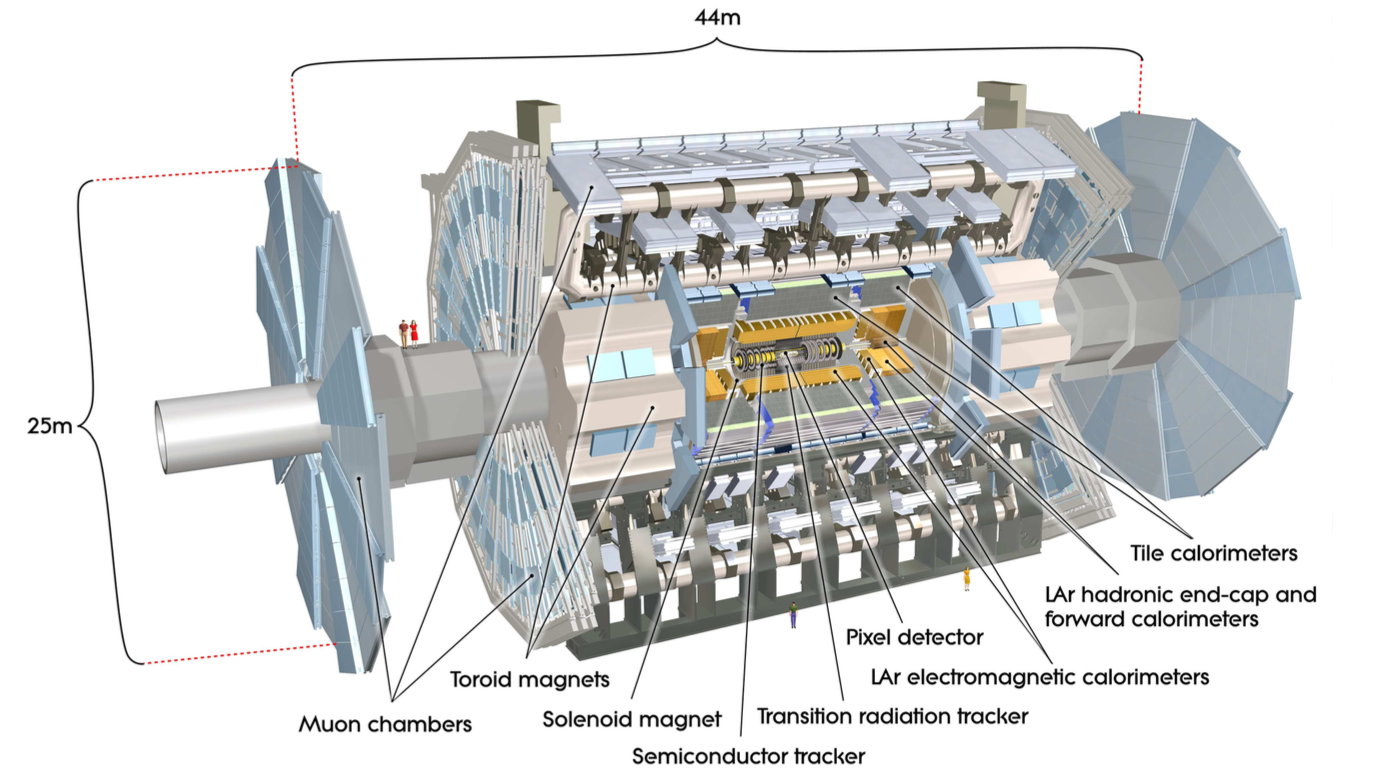
\includegraphics[width=0.95\textwidth]{figures/Atlas/atlas_detector}
    \caption[Diagram of the ATLAS detector]{Diagram of the ATLAS detector, with the major subsystems labeled~\cite{ATLAS}.}
    \label{fig:atlas_detector}
\end{figure}

In the right-handed coordinate system of ATLAS, the IP defines the origin. The beam direction lies along the $z$-axis, transverse to the $x$-$y$ plane. The positive $x$-axis points from the IP to the center of the LHC, while the positive $y$-axis points vertically away from the center of the Earth. The azimuthal angle, $\phi$, circles the beam line from the positive $x$-axis towards the positive $y$-axis, and the polar angle, $\theta$, is measured from the positive $z$-axis.  

It is often more convenient\footnote{
    Differences in rapidity are Lorentz invariant under longitudinal boosts. Since partons in collisions will carry varying fractions of longitudinal momentum, the collision rest frames will have varying boosts. 
} in a hadronic collider to use the rapidity, $y$ (\Eqn{\ref{eqn:rapidity}}), instead of the polar angle. In the massless or highly relativistic limit, the pseudo-rapidity, $\eta$, can be used (\Eqn{\ref{eqn:pseudorapidity}}). Finally, angular distances in $\eta$-$\phi$ space are measured by $\Delta R$ (\Eqn{\ref{eqn:deltar}}).
\begin{eqnarray}
	y &\equiv& \frac{1}{2}\ln\left(\frac{E+p_{z}}{E-p_{z}}\right) \label{eqn:rapidity}  \\
	\eta &\equiv& - \frac{1}{2}\ln \left[\tan\left(\frac{\theta}{2}\right)\right]= \frac{1}{2}\ln\left(\frac{|\boldsymbol{p}|+p_{z}}{|\boldsymbol{p}|-p_{z}}\right) \label{eqn:pseudorapidity} \\
	\Delta R &\equiv& \sqrt{\Delta \eta ^2 +\Delta \phi ^2} \label{eqn:deltar}
\end{eqnarray}

The regions of smallest $|\eta|$ are referred to as the ``central'' or ``barrel'' region. The ``end-cap'' region of the detector bookends the barrel region at larger $|z|$. The largest $|\eta|$ regions, closest to the beam line, are referred to as the ``forward'' region.

%%
\section{Inner Detector}
\label{ch:atlas:id}

The Inner Detector (ID)~\cite{ID_TDR,ID_TDR2,IBL_TDR, ATL-PHYS-PUB-2009-002}, shown in~\Fig{\ref{fig:atlas_id}}, is the subsystem closest to the IP, circling the beam pipe and covering up to $|\eta| = 2.5$. Tasked with untangling the dense jungle of over 1000 particles emanating from the IP in this region every 25 ns, the ID delivers precise charged particle position and momentum measurements. High granularity modules at smaller radii, combined with continuous tracking modules at larger radii, allow for robust pattern recognition and exceptional precision in both $\phi$ and $z$. Additionally, the ID provides electron identification information below $|\eta|=2.0$, for energies between 0.5 and 150 GeV\footnote{
    This is complementary to the electron identification performed in the calorimeters, which uses calorimeter shower shape variables, and particularly aids with low $p_{\rm T}$ electrons.
}. The coverage and spatial resolution of the ID subsystems are detailed in \Tab{\ref{tab:ID_res}}.

\begin{figure}[tp]
    \centering
    \includegraphics[width=0.95\textwidth]{figures/Atlas/atlas_id}
    \caption[Diagram of the ATLAS Inner Detector]{Diagram of the ATLAS Inner Detector~\cite{ATLAS}.}
    \label{fig:atlas_id}
\end{figure}
\begin{table}[tbp]
\caption[Spatial resolution of the ATLAS Inner Detector]{Spatial resolution of the subsystems in the Inner Detector~\cite{ATL-PHYS-PUB-2009-002}.}
\label{tab:ID_res}
\begin{center}
\begin{tabular}{lcccc}
	\hline
	\vbox{\hbox{\strut \textbf{Subsystem}}\hbox{\strut}} & \vbox{\hbox{\strut \textbf{Coverage}}\hbox{\strut }} & \vbox{\hbox{\strut \textbf{Transverse ($R-\phi$)}}\hbox{\strut \textbf{Resolution}[$\mu$m]}} &  \vbox{\hbox{\strut \textbf{Longitudinal ($z$)}}\hbox{\strut \textbf{Resolution}[$\mu$m]}} & \vbox{\hbox{\strut \textbf{Avg. }}\hbox{\strut \textbf{\# Hits}}} \\ \hline\hline
	\textbf{Barrel} \\
	\, IBL   & $|\eta|<2.9$ & $10$ &$75$ &1 \\
	\, Pixel & $|\eta|<2.5$ & $10$ & $115$ & 3\\
	\, SCT & $ |\eta| < 1.5$ &$17$&$580$ & 4 \\
	\, TRT & $|\eta|<1.0$ & $130$&---& 36 \\
	\textbf{Endcap}\\
	\, Pixel & $2.0<|\eta|<2.5$ & $10$  & $115$ (R)  & 3 \\
	\, SCT  & $1.3<|\eta|<2.5$ & $17$  & $580$ (R) & 9 \\
	\, TRT  & $0.8<|\eta|<2.0$ & $130$ & --- & 36 \\
		\hline
\end{tabular}
\end{center}
\end{table}

Multiple high-precision position measurements in the innermost region allow for reconstruction of the particle's path, called a ``track''. Surrounding the ID is a 2 T solenoid magnet, which allows for measurements of charged particle transverse momentum, $p_{\rm T}$, by measuring the curvature of the path\footnote{
    The magnetic field lies along the $z$ axis, thus only the component in the transverse $x$-$y$ plane of the charged particle momentum contributes to the curved track.
}. The reconstructed track can be extrapolated to sub-detectors at larger radii and to vertices near the IP. 

\begin{wrapfigure}{r}{0.55\textwidth}
    \centering
     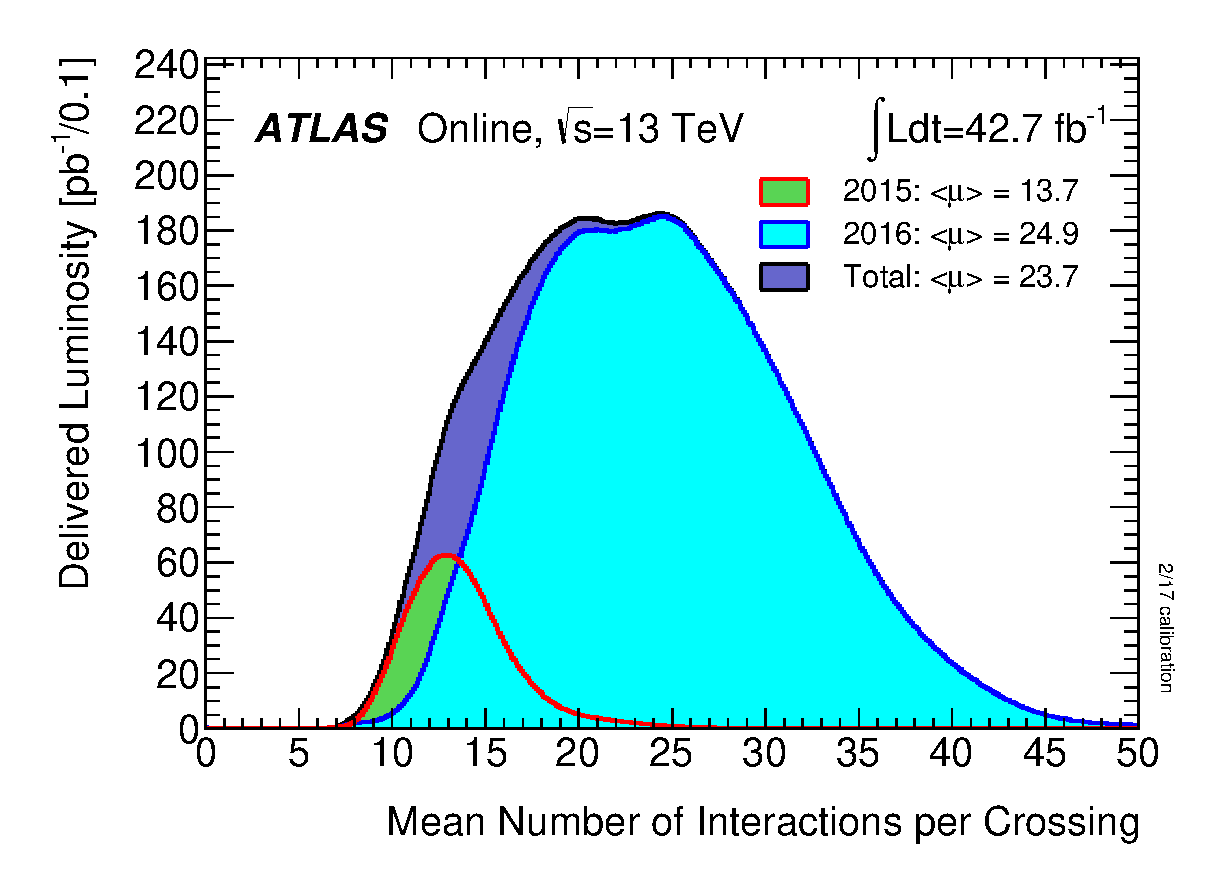
\includegraphics[width=0.53\textwidth]{figures/ATLAS/mu_2015_2016}
     \caption[ATLAS mean interactions per bunch crossing in 2016]{The luminosity weighted average number of interactions per bunch crossing, $\langle\mu\rangle$, for the 2015 and 2016 data taking periods~\cite{Lumi_Public_Run2}.}
     \label{fig:mu_2015_2016}
\end{wrapfigure}

The high luminosity environment at the LHC creates a dense background of overlapping tracks. ``Pileup'' (PU) events occur when there are simultaneous interactions during a bunch crossing, denoted by $\mu$ which reached an average value of 24.9 in 2016~\cite{Lumi_Public_Run2} (\Fig{\ref{fig:mu_2015_2016}}). Consistent and precise vertex identification is essential to mitigate pileup and maintain physics sensitivity. A Z boson candidate event with 25 reconstructed vertices is shown in~\Fig{\ref{fig:25_ver_zmumu}} to illustrate the importance of precise vertex reconstruction. 

The design and layout of the ID reflects a compromise between several competing requirements. The material budget in the tracking volume
%, shown in~\Fig{\ref{fig:id_mat_bud}}, 
should be minimized to reduce scattering and energy loss. However, 
%high rates require close proximity electronics, 
large particle flux requires radiation hardness, and high precision tracking requires a robust, rigid structure. High granularity near the IP must also be balanced with enough tracking volume to accurately measure the curvature of particles. The three layers of the ID attempt to address these design constraints: an innermost Pixel Detector, a Semiconductor Tracker (SCT), and a Transition Radiation Tracker (TRT).  
\begin{figure}[tbp]
    \begin{center}
    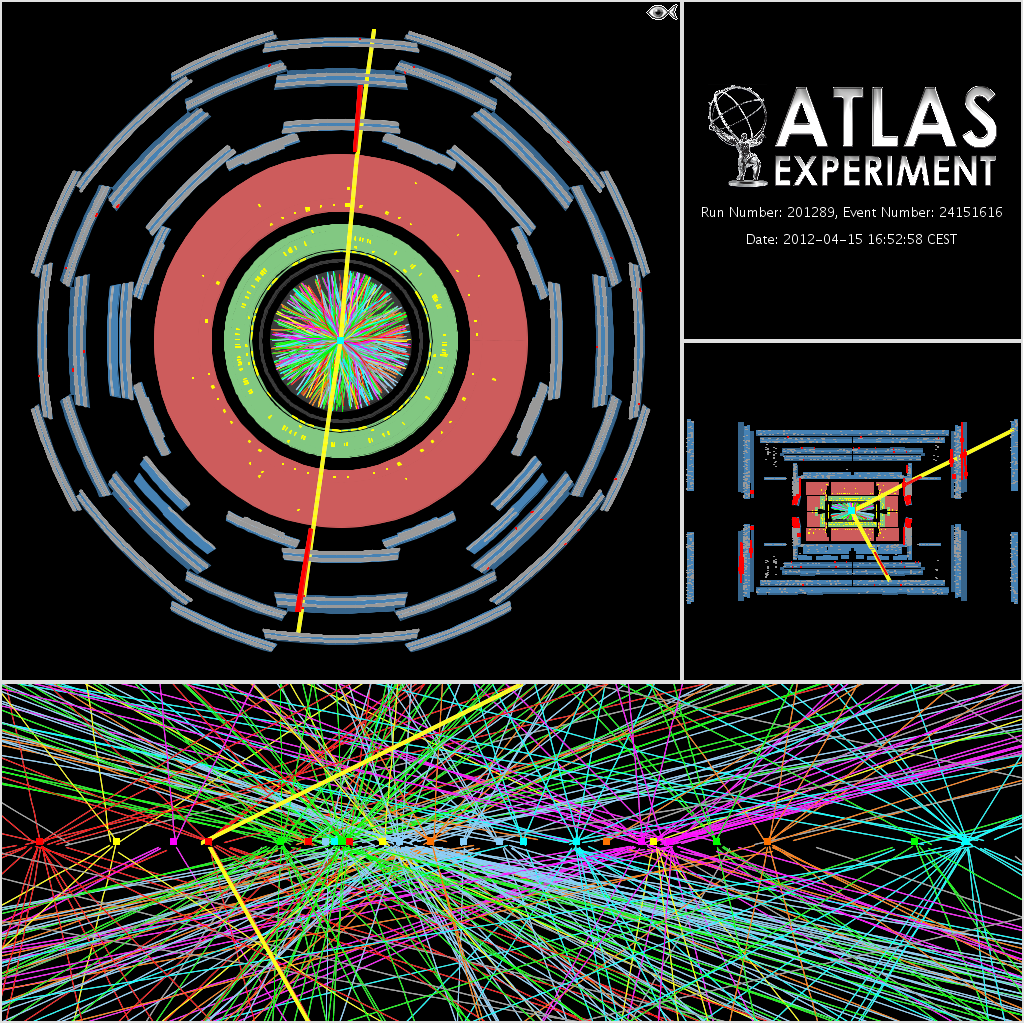
\includegraphics[width=0.8\textwidth]{figures/Atlas/25ver_zmumu}
    \caption[High vertex multiplicity event]{A candidate Z boson event decaying to two muons with 25 reconstructed vertices. This event was recorded on April 15th, 2012 and demonstrates the ATLAS high pileup environment~\cite{25_vertices_z}.}
    \label{fig:25_ver_zmumu}
    \end{center}
\end{figure}
%\begin{figure}[tbp]
%    \centering
%   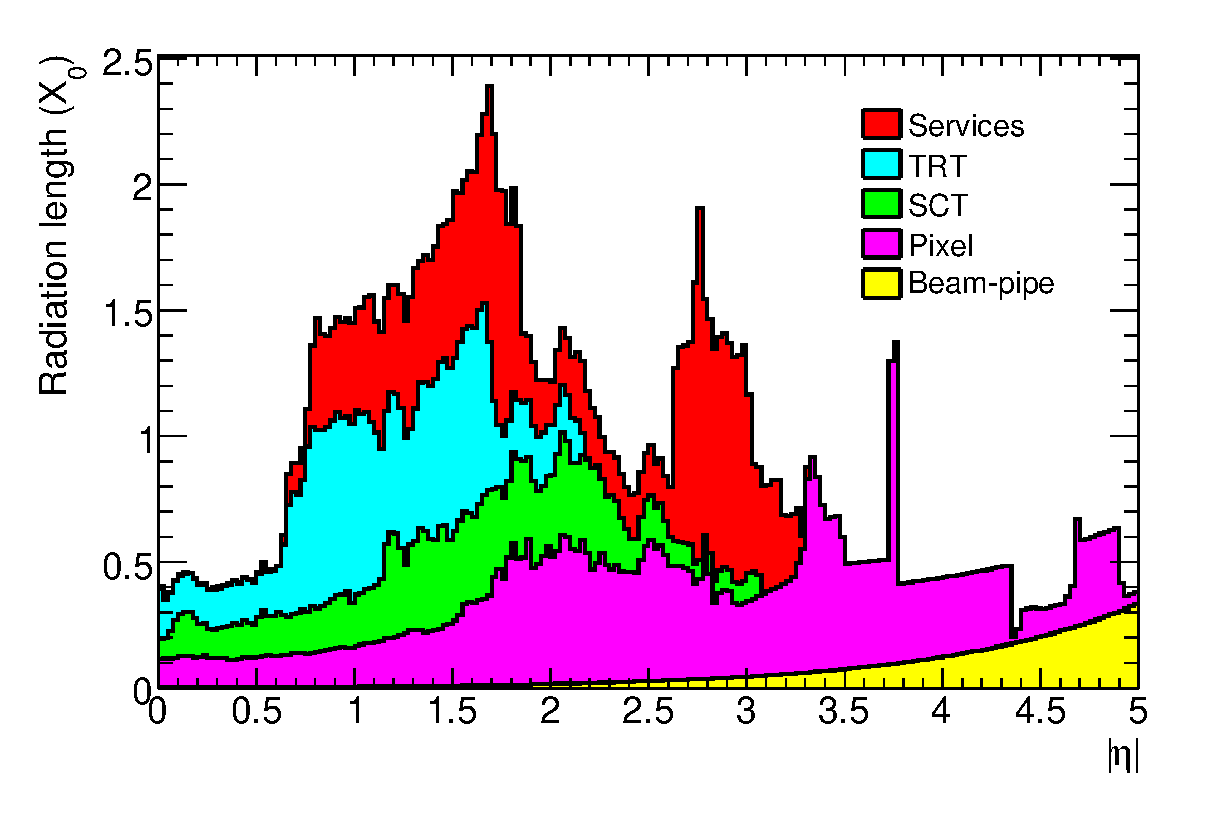
\includegraphics[width=0.58\textwidth]{figures/Atlas/id_mat_bud}
%  \caption[Inner Detector Material Budget]{Material distribution (in radiation lengths $X_0$) of the ID as a function of $|\eta|$, averaged over $\phi$~\cite{ATLAS}.}
% \label{fig:id_mat_bud}
%\end{figure} 


%
\subsection{Pixel Detector and Insertable B-Layer}
The primary objective of the Pixel Detector is to provide accurate impact parameter resolution, vertex identification, and short-lived particle identification for objects such as $b$-quarks and $\tau$-leptons.

The sensors~\cite{Pixel_Sensors} in the Pixel Detector are fabricated on silicon wafers using bipolar diodes on an n-type bulk. The readout side of the sensor uses n$^+$ doping\footnote{
	The\,$^{+}$ here denotes a relatively large amount of doping, near degenerate levels.
}, while the back side has an asymmetrically depleted p$^+$-n junction creating a reverse bias through the entire bulk. Particles passing through the bulk ionize it, allowing charge carriers to be collected on the sensor. A ``hit'' is registered if the amount of charge accumulated surpasses a threshold.

%Irradiation of the sensors eventually will lead to a type conversion of the bulk from n to p. Depletion begins on the p$^+$-n junction, lowering the effective doping until type conversion. Then, the junction will be on the readout (n) side isolating the pixels which allows operation below the depletion voltage.
%\footnote{The voltage required to fully deplete the bulk of charge carriers. Operating below this voltage is possible but brings about signal degradation.} 

The original Pixel Detector consists of three cylindrical layers,
%\footnote{The innermost layer, layer 0, is also sometimes called the B-layer or barrel layer. The two other layers are just known as layer 1 and layer 2.} 
concentric with the beam pipe, and three disk layers in the forward regions (both A and C side) perpendicular to the beam pipe. In 2014, a fourth innermost layer called the Insertable B-Layer (IBL) was installed, along with a new smaller radius beryllium beam pipe.
%\footnote{The radius was decreased from 29 mm to 25 mm.}
The spatial layout of the Pixel and IBL detectors is summarized in \Tab{\ref{tab:pixel_config}}. For clarity, descriptions of the Pixel Detector refer to the original three layers, whereas the IBL will be explicitly written to denote the new innermost layer.

The design and insertion of the IBL was meant to ready the ID for conditions up to the start of the High Luminosity LHC (HL-LHC), at which point ATLAS is projected to have recorded 300 fb$^{-1}$ of data. As modules in the innermost Pixel layer (B-layer) age, they may begin failing. Additionally, the peak luminosity will reach twice the design value of $10^{34}$ cm$^2$s$^{-1}$, leading to high PU\footnote{
	Projected $\langle\mu\rangle\sim 60$.
} and readout inefficiencies. The IBL serves to add robustness and redundancy to the tracking capabilities of the Pixel Detector. Improved performance at low $p_{\rm T}$ helps secure excellent tracking, impact parameter resolution, and $b$-tagging efficiency in a high PU environment~\cite{ID_RUN2_PROC}. 


\begin{table}[tbp]
\caption[Summary of ATLAS Pixel Detector configuration]{Spatial configuration and extent of the Pixel Detector and IBL system~\cite{IBL_TDR}.}
\label{tab:pixel_config}
\begin{center}
\begin{tabular}{lccccc}
	\hline
	\vbox{\hbox{\strut \textbf{Component}}\hbox{\strut}} & \vbox{\hbox{\strut \textbf{Radial}}\hbox{\strut  \textbf{Extension} [mm]}} & \vbox{\hbox{\strut \textbf{Length}}\hbox{\strut [mm]}} & \textbf{\vbox{\hbox{\strut Staves /}\hbox{\strut Sectors}}} & \vbox{\hbox{\strut \textbf{Modules}}\hbox{\strut }} & \vbox{\hbox{\strut \textbf{Pixels}}\hbox{\strut (x$10^6$)}}\\ \hline\hline
	Beam  Pipe & $25 < R < 29$ & & & & \\ \\
	\textbf{IBL} \\
	 & $\langle R\rangle = 33.25$ & $|Z| < 332$ & 14 & 224 & 12 \\ \\
	 \textbf{Pixel} \\
	 B-layer & $\langle R\rangle = 50.5$ & $|Z| < 400.5$  &22 & 286 & 13.2 \\
	 Layer 1 & $\langle R\rangle = 88.5$ & $ |Z| < 400.5$ & 38 & 494 & 22.8 \\
	 Layer 2 & $\langle R\rangle= 122.5$ & $|Z|< 400.5$  & 52 & 676 & 31.2 \\
	 Disk 1 & $88.8 < R < 149.6$ & $\langle Z\rangle = 495$ & $8\times2$ & $48\times2$ & 4.4 \\
	 Disk 2 & $88.8 < R < 149.6$ & $\langle Z\rangle = 580$ & $8\times2$ & $48\times2$ & 4.4 \\
	Disk 3 & $88.8 < R < 149.6$ & $\langle Z\rangle = 650$ & $8\times2$ & $48\times2$ & 4.4 \\
	&&&&\em{Pixel Total}& $80.4$\\
	\hline
\end{tabular}
\end{center}
\end{table}

%\begin{figure}[tbp]
%\begin{center}
%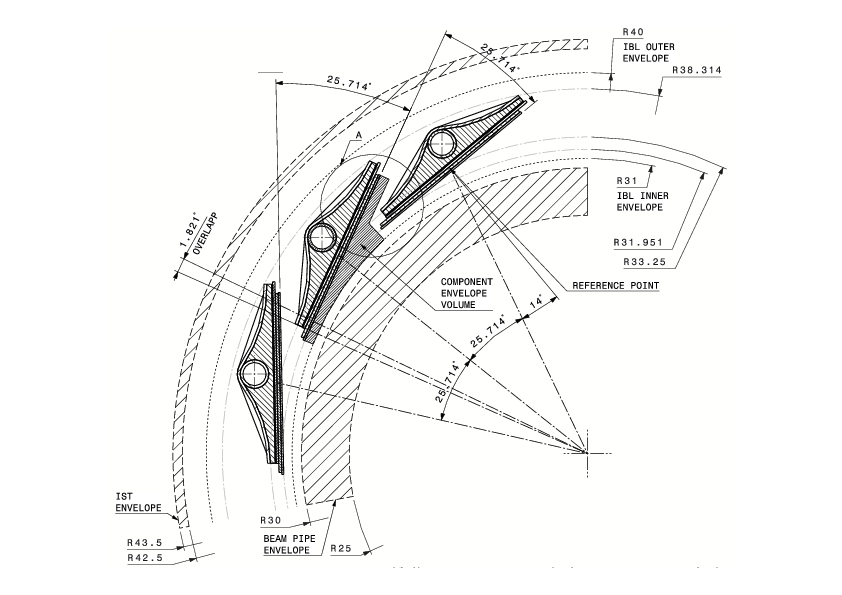
\includegraphics[width=.85\linewidth]{figures/ATLAS/ibl_layout_rev}
%\caption[IBL layout]{Layout of the IBL in the $R-\phi$ plane~\cite{IBL_TDR}.}
%\label{fig:ibl_layout}
%\end{center}
%\end{figure}

The IBL consists of approximately 12 million pixel channels. The main structure is comprised of 14 carbon-fibre cooling supports, called staves, set at a $14^{\circ}$ azimuthal tilt.
%\footnote{Measured as the tangent to the stave surface in the plane perpendicular to the cylinder axis.} (see \Fig{\ref{fig:ibl_layout}}) 
%The light carbon-fibre staves allow for a tiny 1.54\% $X_0$
%\footnote{Radiation length, average path in material for relativistic charged particle to lose 67\% of its energy.} 
%footprint. Each stave measures 2 cm (width) $\times$ 64 cm (length) and covers  a range in $\eta$ of approximately $\pm 3$. 
A stave holds 32 front-end chips (FE-I4) with 130 nm CMOS technology that are bump-bonded
%\footnote{Either electroplated solder (PbSn) or evaporative indium methods are used to attach the integrated circuit to the substrate. } 
to silicon sensors with 26,880 pixels each. 
%Each sensor has 80 columns $\times$ 336 rows of pixel cells (50 $\mu$m $\times$ 250 $\mu$m), for a total of 26,880 pixels per sensor. 
The central part of the stave utilizes $200 \mu$m thick planar n$^+$-in-n silicon sensors, while the forward ends of the stave carry new 3D n-in-p sensors with electrodes passing through the bulk. The $230\,\mu$m thick 3D sensors are more robust to irradiation with respect to the planar sensors. The transverse resolution of the IBL is $10\,\mu$m in $R-\phi$, while the longitudinal resolution is $75\,\mu$m in $z$.

Overall, the Pixel Detector has over 80 million pixel channels. In the cylindrical barrel region $|\eta|<2.5$, Pixel support staves are set at a $20^{\circ}$ azimuthal tilt.
% and a total material budget of 3\% $X_0$. 
%, the B-layer, layer 1, and layer 2 have 22, 38, and 52 cooling support staves respectively, each set at a $20^{\circ}$ azimuthal tilt. 
Each stave holds 13 modules with 16 front-end chips (FE-I3) with 250 nm CMOS technology that are bump bonded to silicon sensors with 46,080 pixels each. 
%The 250\,$\mu$m thick planar n$^+$-in-n sensors feature 18 columns $\times$ 160 rows of pixel cells ($50 \mu$m $\times$ $400 \mu$m), for a total of 46,080 pixels per sensor. 
The three disks on each end-cap cover $2.0< |\eta| < 2.5$ and are split into 8 sectors\footnote{
A sector is the end-cap analogue of staves in the barrel region.} 
with 6 sensors each (identical to those in the barrel). The Pixel Detector has a transverse resolution of $10\,\mu$m in $R-\phi$, and a longitudinal resolution of $115\,\mu$m in $z$ ($R$) in the barrel (end-cap) region. 

%
\subsection{Semiconductor Tracker}

The Semiconductor Tracker (SCT) provides on average four precise position measurements per track at intermediate radial distances in order to guarantee excellent track reconstruction and charged particle \pt resolution.

Sitting at a farther distance from the IP, the SCT~\cite{SCT_paper} has relaxed radiation hardness and spatial resolution requirements. In contrast with the Pixel Detector, therefore, the SCT uses AC-coupled single-sided silicon micro-strips with p$^+$ strip implants in an n-type bulk, to control for costs and reliability with over 63 m$^2$ of silicon. 

\begin{figure}[tbp]
\begin{center}
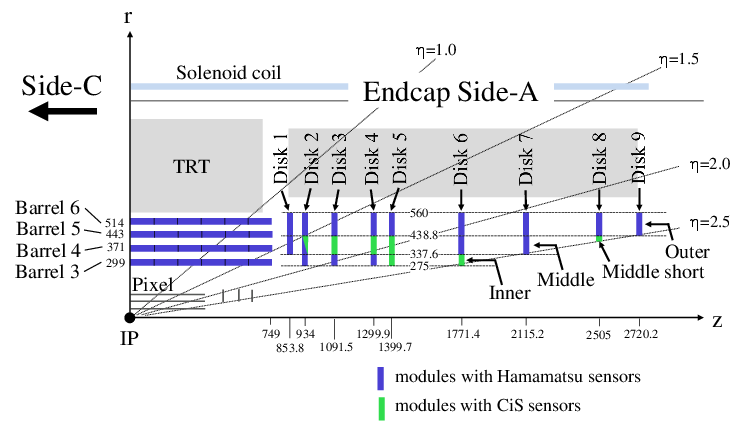
\includegraphics[width=.9\linewidth]{figures/ATLAS/SCT_Quadrant}
\caption[Semiconductor Tracker layout]{Layout of the SCT in the $R-z$ plane~\cite{SCT_paper}.}
\label{fig:sct_layout}
\end{center}
\end{figure}

The layout of the SCT, shown in \Fig{\ref{fig:sct_layout}}, is similar to that of the Pixel Detector: there are four concentric barrel layers
%\footnote{The numbering scheme is B3, B4, B5, B6.} 
positioned between radii $R_3=299$\,mm and $R_6=514$\,mm, and nine forward disks with up to three rings on either end-cap situated between $z_1=853.8$\,mm and $z_9=2720.2$\,mm. Over 6.3 million channels, covering $|\eta|<2.5$, are spread over 4088 modules that tile the SCT: 2112 rectangular modules in the barrel at an $11^{\circ}$ tilt, and 1976 trapezoidal modules in the disks. Most modules feature two 285\,$\mu$m thick sensors back-to-back with a stereo angle of 40 mrad. A layer will thus register two strip measurements, which are combined to obtain the $z$ position and create a space-point. Each sensor has 768 strips with a pitch of 80\,$\mu$m
%\footnote{The wedge modules in the disks have varying pitches between $50-90\,\mu$m.} 
and length of 63\,mm. Two sensors on each side of the module are daisy-chained to create a total strip length of 126\,mm.  The SCT has a transverse resolution of $17\,\mu$m in $R-\phi$, and a longitudinal resolution of $580\,\mu$m in $z$ (R) in the barrel (end-cap) region.



%
%\clearpage
\subsection{Transition Radiation Tracker}
The Transition Radiation Tracker (TRT) provides continuous tracking for particles within $|\eta|<2$, by registering on average 36 hits per track. Additionally, the TRT is capable of particle identification by differentiating between electrons and hadrons by using transition radiation.

The TRT is comprised of approximately 300,000 gas-filled polyimide drift tubes~\cite{TRT_sensors}, called straw tubes, of diameter 4\,mm. In the barrel, 52,544 straws with a length of 144\,cm are positioned parallel to the beam axis  and cover $|\eta| < 1$. Each end-cap features 122,880 straws aligned radially on two types of wheels with a length of 37\,cm, covering $1<|\eta|<2$. The spatial extent of the TRT is shown in \Tab{\ref{tab:trt_layout}}.

\begin{table}[bh]
\begin{center}
\caption[Transition Radiation Tracker spatial layout]{Layout of the barrel and end-cap modules of the TRT.}
\label{tab:trt_layout}
\begin{tabular}{llllll}
\hline
\textbf{Component} & $|z_{\text{min}}|$ [mm]& $|z_{\text{max}}|$ [mm]& $|R_{\text{min}}|$ [mm]& $|R_{\text{max}}|$ [mm] & \textbf{Straws} \\ \hline\hline
TRT barrel & 0 & 712 & 563 & 1,066 & 52,544\\
TRT end-cap & 848 & 2710 & 644 & 1,004 & 122,880 \\ 
\hline
\end{tabular}
\end{center}
\end{table}

%\begin{figure}[htbp]

%\end{figure}

The walls of the straw tubes are made with two bonded 35\,$\mu$m film layers
%\footnote{The film consists of a 25\,$\mu$m thick Kapton film, coated with a 0.2\,$\mu$m Al-deposit and 5-6\,$\mu$m thick graphite-polyimide layer. The other side is coated with 4-5\,$\mu$m thick polyurethane sealant layer.} 
reinforced with carbon fibres. Through the center of each straw tube is a grounded 31\,$\mu$m diameter gold-plated
%\footnote{Approximately 0.5-0.7\,$\mu$m thick.} 
tungsten wire which functions as an anode. The walls of the straws are kept at a -1.53\,kV potential and act as the cathode. The straws are filled with a gaseous mixture of 70\% Xe, 27\% CO$_2$, and 3\% O$_2$.
%\footnote{In Run-2, Ar replaced Xe in straws with gas leaks. Ar provides similar tracking performance; however, it detects transition radiation more poorly than Xe in the operational energy range.}
The volume between each straw is filled with polymer fibres (foils) in the barrel (end-cap) region to create transition radiation.

As charged particles pass through the TRT, the gas in the straws is ionized. The free electrons drift along the lines of the applied potential and are collected on the anode, where the readout signal is compared to a threshold.  By measuring the drift time of particles in the TRT, the distance to the wire from the particle, or drift distance, can be inferred, as depicted in~\Fig{\ref{fig:trt_drift}}. The drift time measurement provides an inherent transverse ($R-\phi$) spatial resolution of 130\,$\mu$m per straw.

\begin{wrapfigure}{r}{.55\textwidth}
\begin{center}
	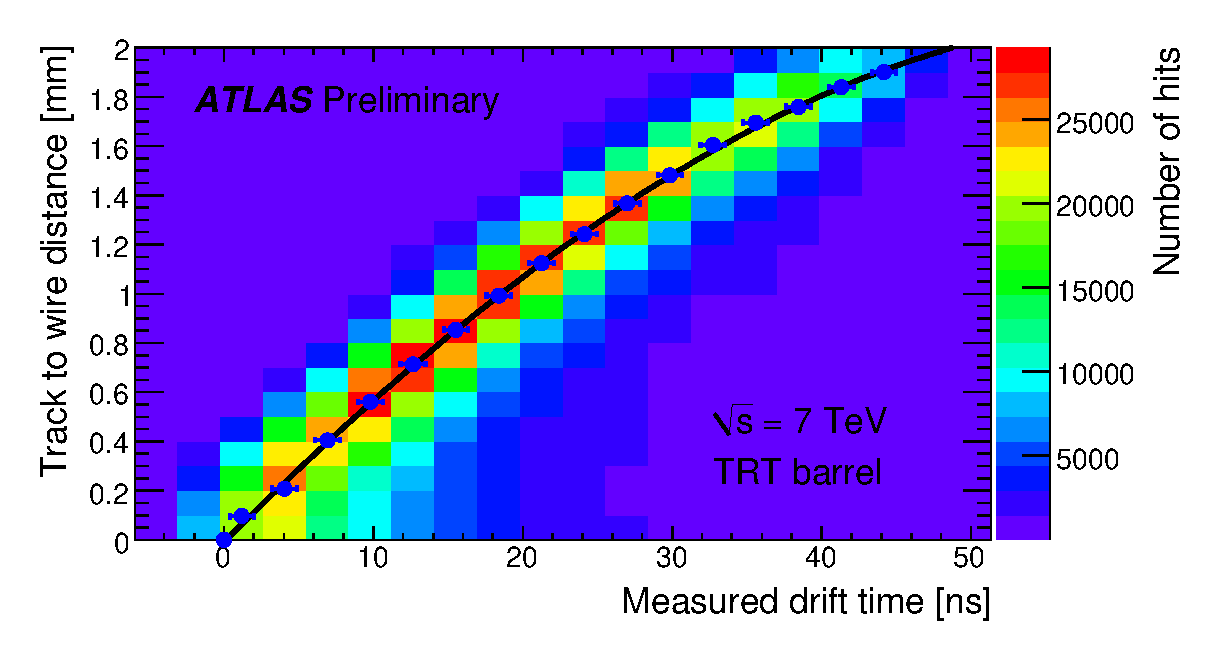
\includegraphics[width=.99\linewidth]{figures/ATLAS/trt_drift}
	\caption[Transition Radiation Tracker wire impact parameter vs drift time]{Using the drift time, the distance from the track to the wire can be inferred. The dependency of the drift radius on measured drift time can be fit with a third order polynomial~\cite{trt_twiki}.}
	\label{fig:trt_drift}
\end{center}
\end{wrapfigure}

Low energy transition radiation is emitted by relativistic charged particles as they traverse a boundary in which the two mediums exhibit different dielectric permittivities. The space filling polymer fibres and foils allow for such radiation to be produced in the TRT. The transition radiation photons are absorbed by the Xe gas in the straws producing a stronger signal response. The amount of transition radiation detected can be used to differentiate
%\footnote{The amount of radiation is proportional to the relativistic factor, $\gamma=E/m$. Electrons will thus have a much stronger response than hadrons.} 
electrons from hadrons, through the use of a second higher readout threshold. 


%%
\section{Calorimetry}

The ATLAS calorimeters~\cite{LAr_TDR,Tile_TDR}, shown in~\Fig{\ref{fig:cal_layout}}, surround the ID and solenoid magnet and aim to fully absorb and provide precise measurements of electrons, photons, jets, and \MET over the range $|\eta|<4.9$. The Liquid Argon (LAr) and Tile Calorimeters are sampling calorimeters: dense layers (absorbers) which induce particle showers alternate with active layers which measure the deposited energy\footnote{
	Since some energy is deposited in the absorbers, the total energy must be estimated from the ``sampled" shower energy in the active layers.
}.

\begin{figure}[tbp]
\begin{center}
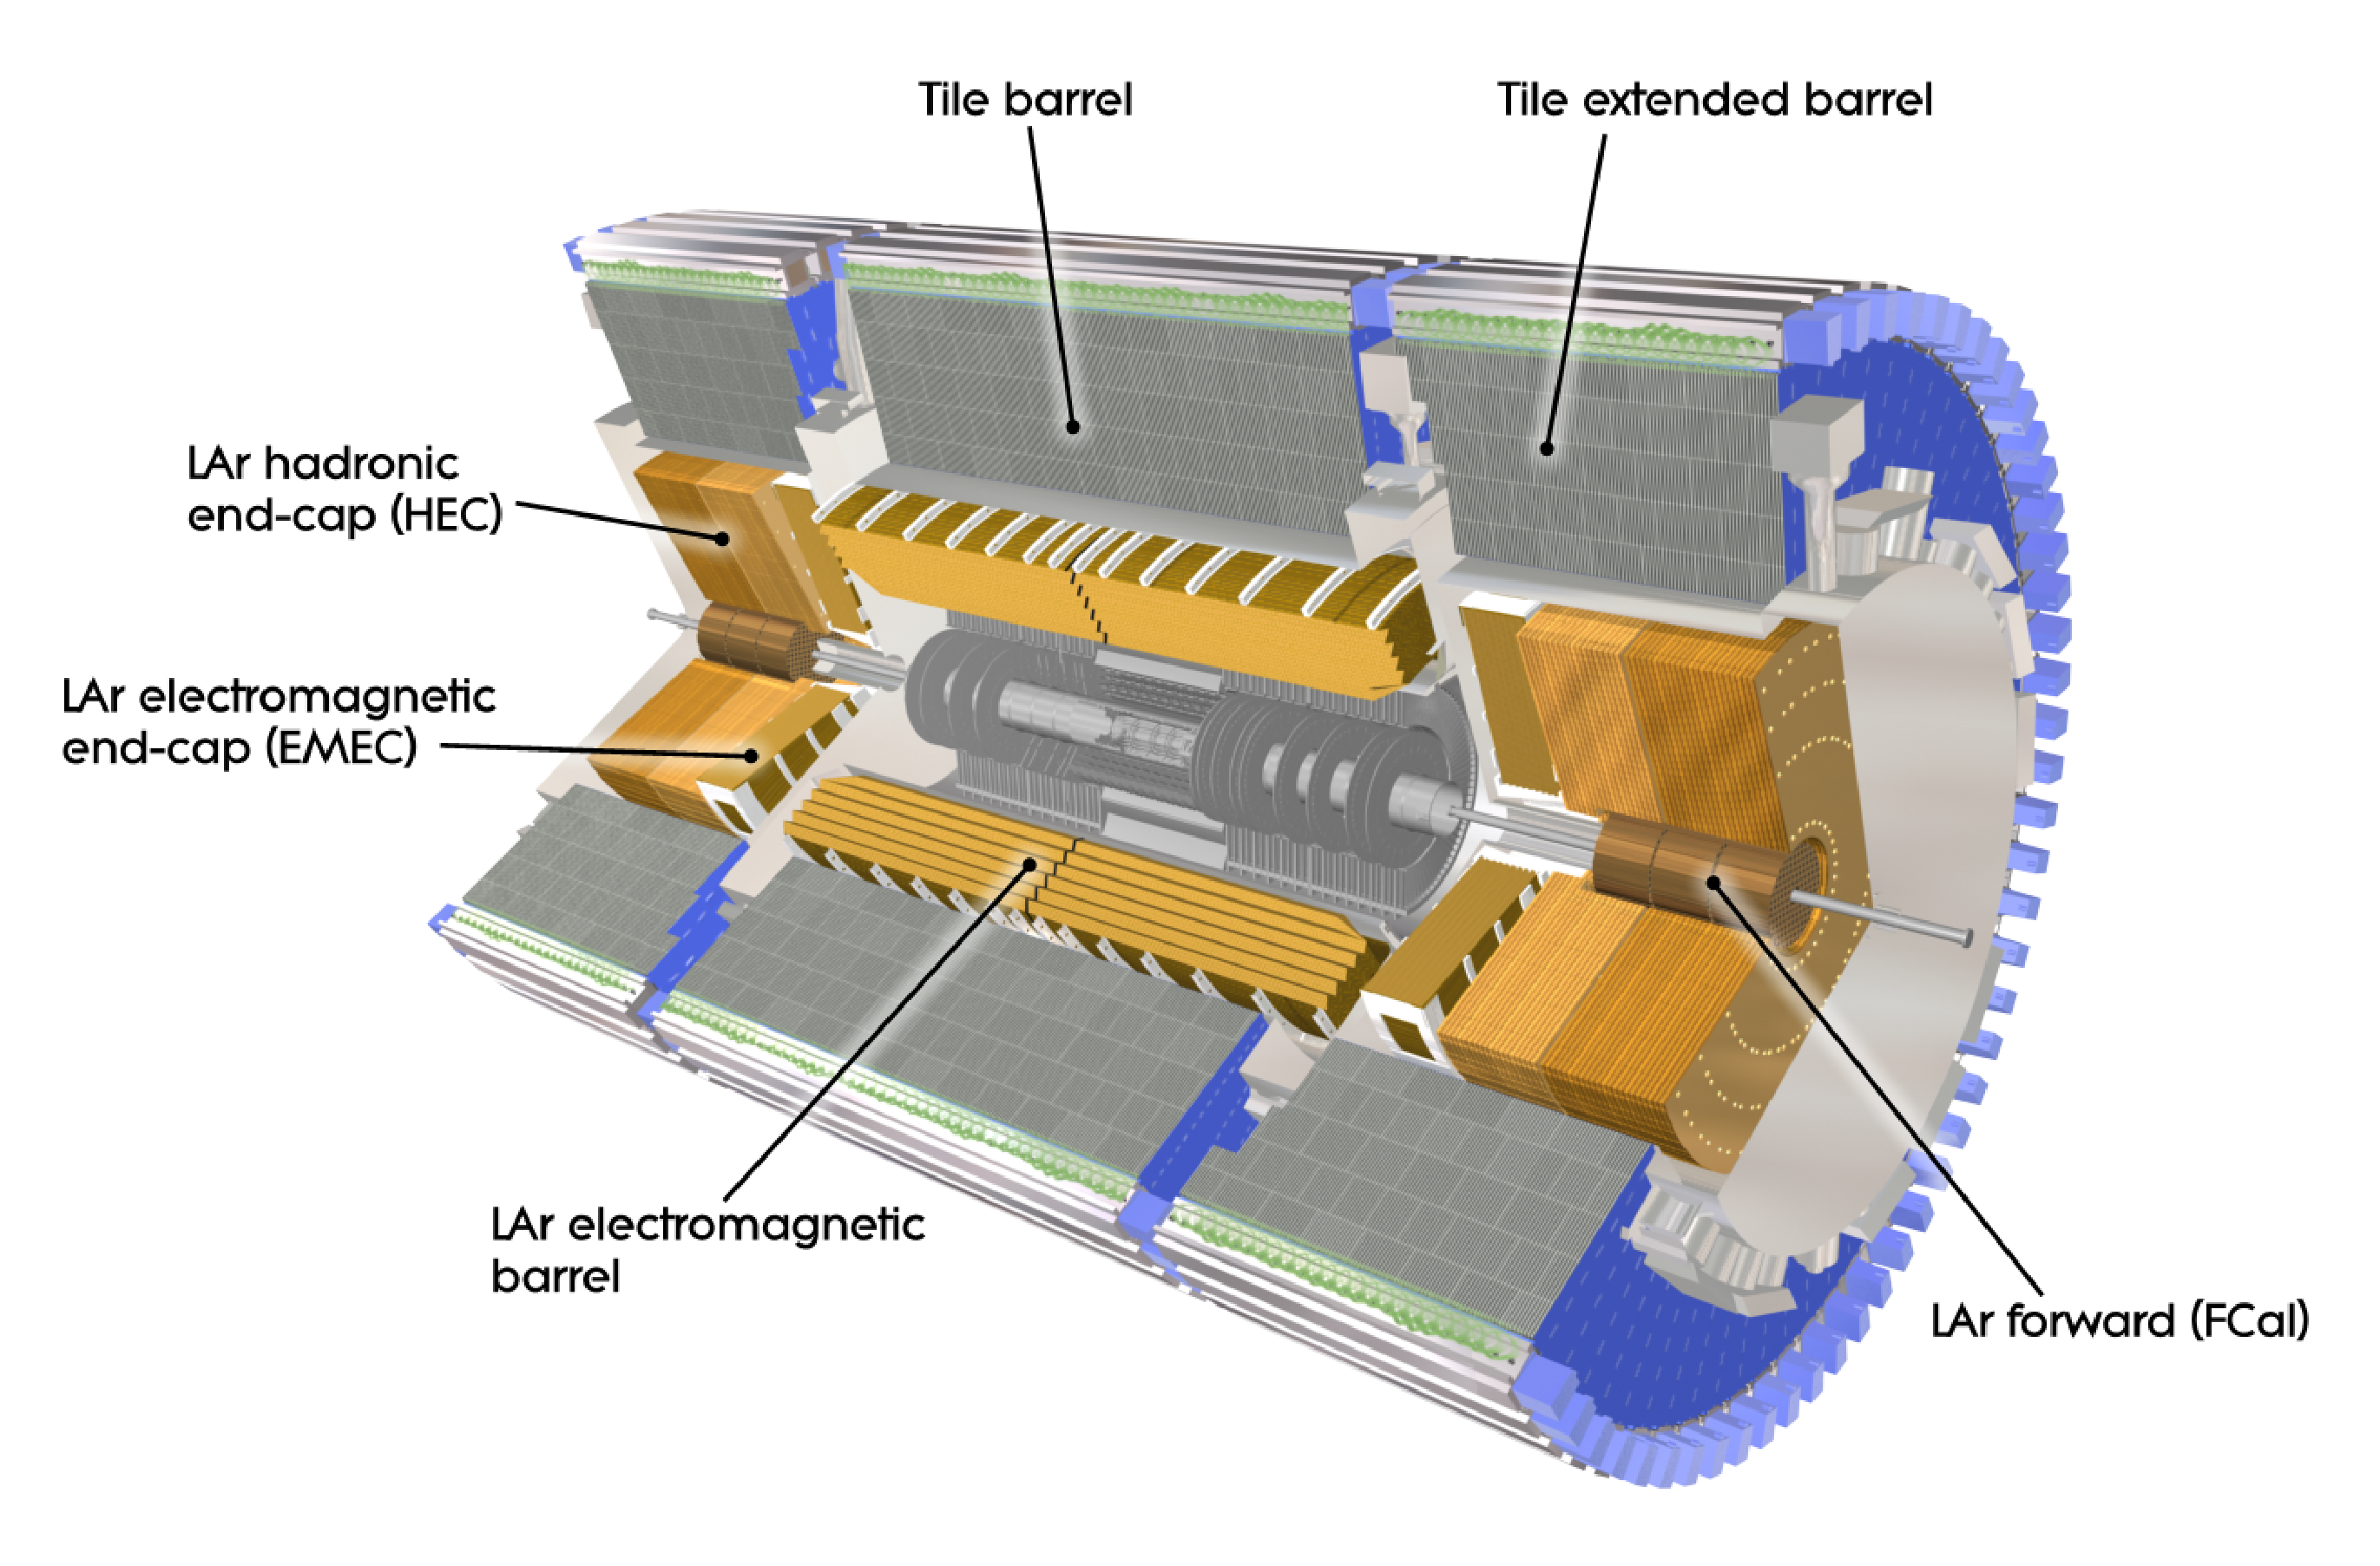
\includegraphics[width=0.8\textwidth]{figures/ATLAS/calorimeter_layout}
\caption[Layout of Liquid Argon and Tile calorimters]{Diagram of the Liquid Argon and Tile Calorimeters which sit outside the Inner Detector and solenoid magnet~\cite{ATLAS}.}
\label{fig:cal_layout}
\end{center}
\end{figure}

The particle showers produced from electromagnetic (EM) particles and those produced from hadronic particles behave differently; thus, two types of calorimeters (EM and hadronic) are designed to cater to each  shower type. LAr EM calorimeters cover $|\eta|<3.2$, LAr hadronic calorimeters cover $1.5<|\eta|<4.9$, and Tile hadronic calorimeters cover $|\eta|<1.7$. Since hadronic showers penetrate deeper than EM showers, the EM calorimeters are placed before the hadronic calorimeters. To characterize the thickness of a material as seen by the EM radiation, the radiation length, $X_0$, measures both the average distance required to lower high energy electrons to $1/e$ times its initial energy via Bremsstrahlung, and also $7/9$ the mean free path for high energy photons to undergo pair production. For hadronic calorimeters, the nuclear interaction length, $\lambda$, measures the average distance traveled by a hadron before interacting with a nucleus.

Each type of calorimeter optimizes separately the choice of material and thickness for the absorber and active layers, as well as the cell size. If particle showers are not fully contained in the calorimeters, some shower particles may penetrate the surrounding Muon Spectrometer, known as ``punch-through''. To prevent punch-through\footnote{
	The goal is two-fold: (1) calorimeter objects which reach the muon spectrometer can induce fake muon rates, and (2) an accurate missing transverse energy measurement requires containment of the full EM and hadronic showers.
}, the total thickness of the EM calorimeters, shown in~\Fig{\ref{fig:x0_cal}}, is approximately $22\,X_0$ in the barrel and $24\,X_0$ in the end-cap region, while the total thickness of the hadronic calorimeters, shown in~\Fig{\ref{fig:lambda_cal}}, is approximately $10\,\lambda$. 

\begin{figure}[htbp]
\begin{center}
\subfloat[]{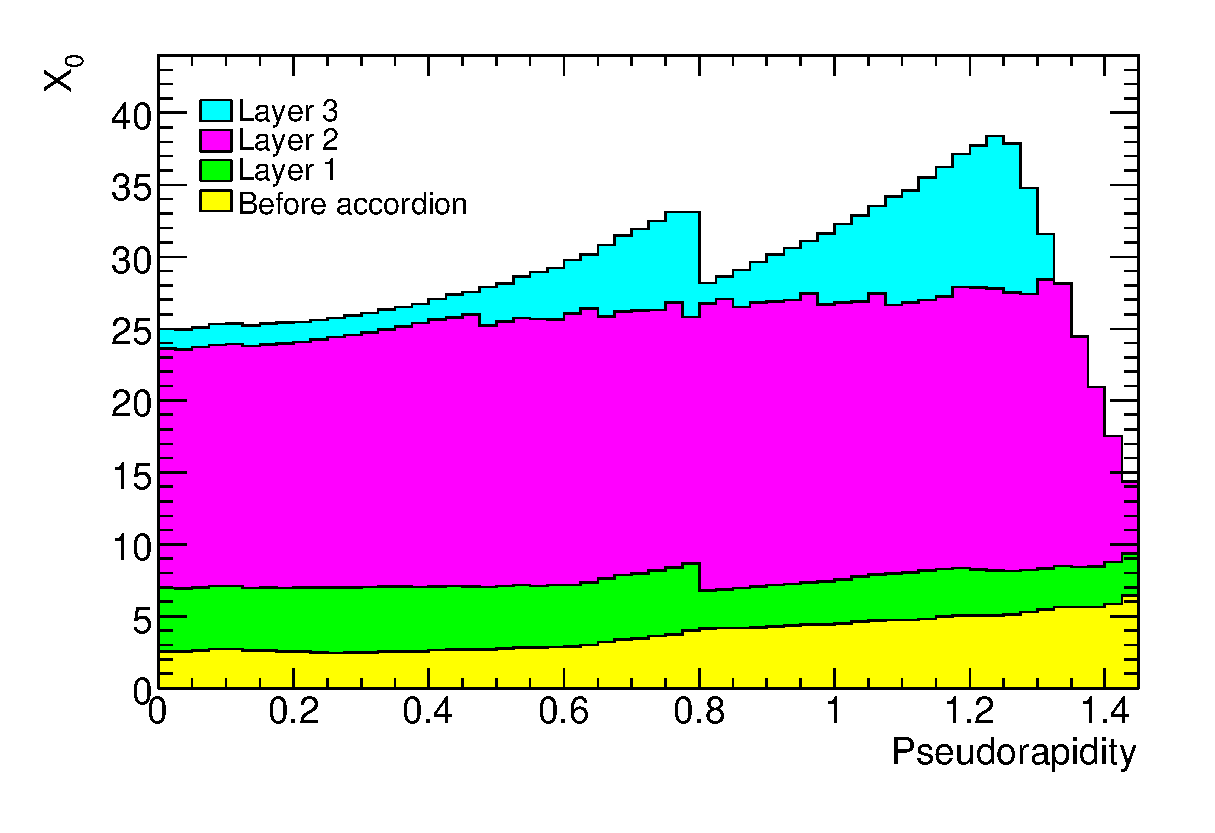
\includegraphics[width=0.49\textwidth]{figures/ATLAS/x0_barrel}\label{fig:x0_cala}}
\subfloat[]{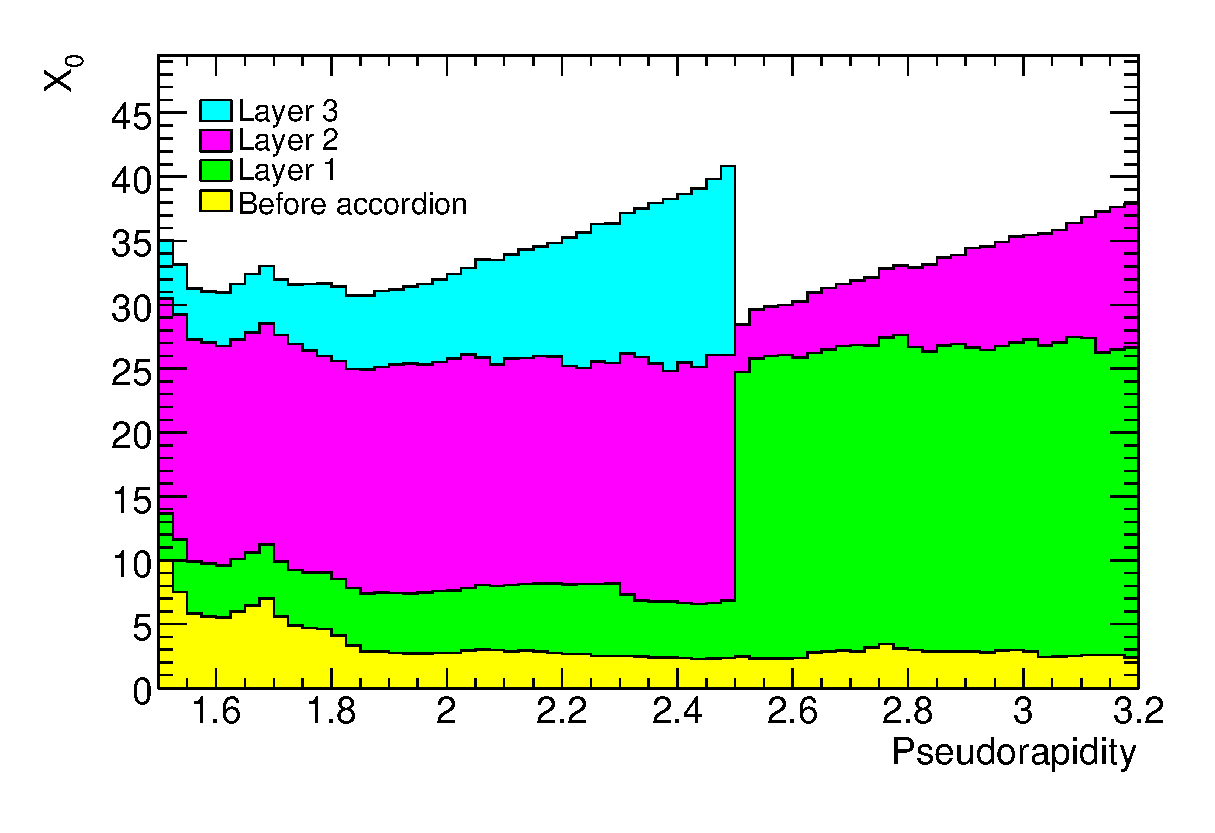
\includegraphics[width=0.49\textwidth]{figures/ATLAS/x0_endcap}\label{fig:x0_calb}}
\caption[Radiation lengths in ATLAS electromagnetic calorimeters]{Total thickness in radiation lengths, $X_0$, of the EM calorimeters in \protect\subref{fig:x0_cala} the barrel and \protect\subref{fig:x0_calb} the end-cap region~\cite{ATLAS}.}
\label{fig:x0_cal}
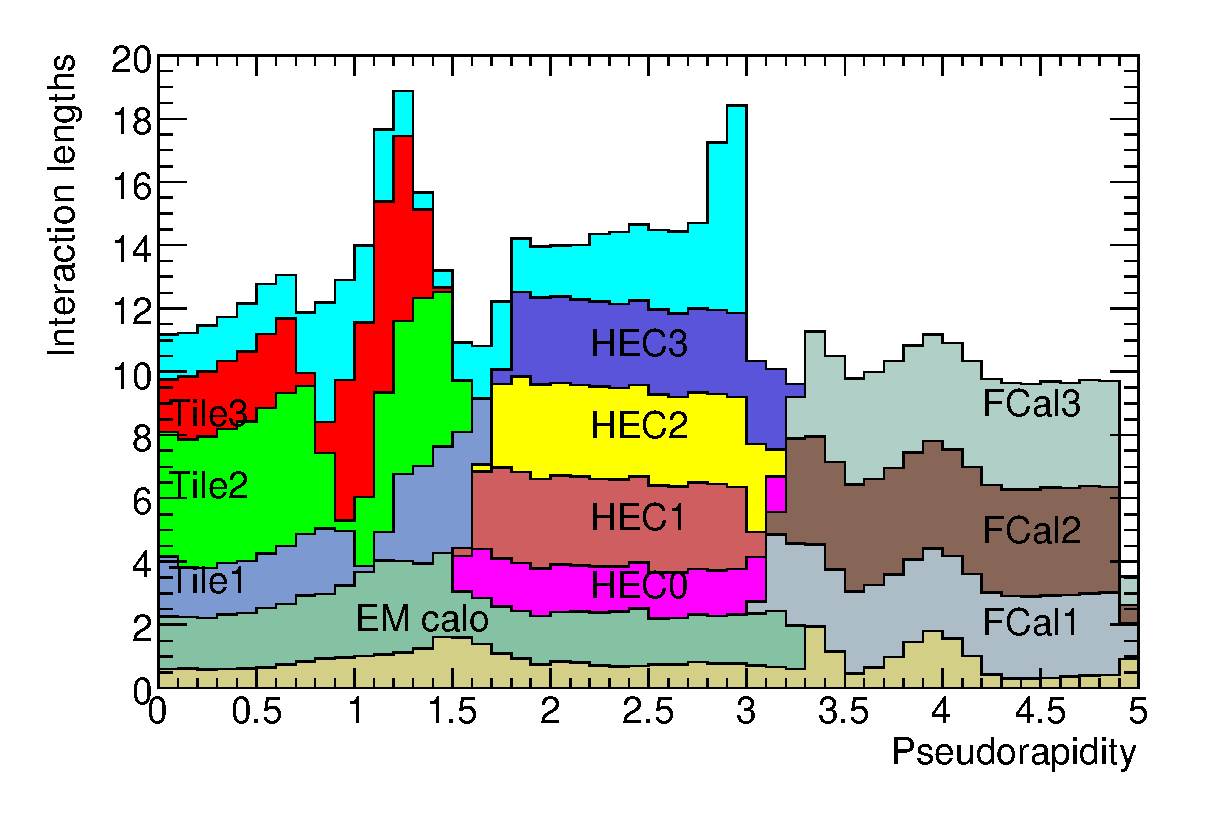
\includegraphics[width=0.8\textwidth]{figures/ATLAS/lambda_cal}
\caption[Interaction lengths in ATLAS calorimeters]{Total thickness in nuclear interaction lengths, $\lambda$, of the ATLAS calorimeters~\cite{ATLAS}.}
\label{fig:lambda_cal}
\end{center}
\end{figure}

%
\subsection{Particle Showers}
\label{ch:atlas:particle_showers}
The calorimeters measure energy of an incoming particle by sampling the energy of the induced particle showers. EM and hadronic showers involve different physics processes and therefore develop differently in the detector\cite{pdg_2017}. 

Electrons, positrons, and photons produce EM showers: energetic electrons radiate Bremsstrahlung photons, while energetic photons convert to electron-positron pairs when traversing dense material. The longitudinal depth of an EM shower is expressed in terms of the radiation length and critical energy, $E_c$\footnote{
	The critical energy $E_c\propto \frac{1}{Z}$ measures the energy at which losses from ionization (logarithmic with energy) are comparable to losses from Bremstrahlung (linear with energy), above which Bremstrahlung dominates. The radiation length $X_0\propto Z(Z+1)$ \cite{pdg_2017}. 
}, in \Eqn{\ref{eq:x0}}.
\begin{equation}
	X = X_0\frac{\ln\left(E_0/E_c\right)}{\ln 2}
	\label{eq:x0}
\end{equation}

Hadronic showers involve processes including hadron production from QCD radiation, pion decays, and de-exciting nuclei. Approximately half of the energy of the hadron is transferred to secondary hadrons produced in the shower. About one third of the energy dissipated in the hadronic shower is via neutral pions which decay via $\pi^0\to\gamma\gamma$ and produce an EM component of the shower. Additionally, particles may interact with the nuclei in the absorber in a variety of nuclear processes, which then produce additional particles near the MeV scale.  The longitudinal depth of the hadronic shower scales with the nuclear interaction length, $\lambda\propto A^{\frac{1}{3}}$. 


%
\subsection{Liquid Argon Calorimeter}

With over 180,000 channels, the LAr calorimeters consist of both EM and hadronic modules. The LAr EM calorimeters are divided into the barrel (EMB) region covering $|\eta|<1.475$ and two coaxial end-cap regions (EMEC) covering $1.375<|\eta|<3.2$. The EMB consists of two cylindrical half-barrels, each 3.2\,m in length with an inner (outer) diameter of $2.8$\,m ($4$\,m). The wheels of the EMEC are 63\,cm thick and extend radially between $R=330$\,mm and $R=2098$\,mm.  Each end-cap wheel is divided into an inner wheel from $1.375<|\eta|<1.5$ and an outer wheel from $1.5<|\eta|<3.2$. Accordion-shaped lead absorber plates alternate with similarly shaped copper-kapton electrodes, with liquid argon filling the bulk as the active medium. The accordion structure ensures complete $\phi$ coverage with no gaps. In the barrel the accordion folds are axial while in the end-cap they are radial. The angle and amplitude of the folds varies with radius to ensure constant gaps.

Incident particles shower in the absorber layer, and ionize the LAr. The electrodes are kept near $2$\,kV to allow the electrons to drift through 2.1\,mm gaps on either side of the electrodes, which corresponds to a relatively slow drift time of $450$\,ns. The electrodes collect a triangular pulse which is then shaped and sampled once every 25\,ns, as shown in~\Fig{\ref{fig:lar_pulse}}. In Run I (Run II), five (four) samples of the shaped pulse were read out to reconstruct the time and energy of the pulse. As the pulse spans multiple bunch crossings, care must be taken to account for out-of-time PU due to collisions in nearby bunches.

%\begin{figure}[tbp]
\begin{wrapfigure}{r}{0.52\textwidth}
\begin{center}
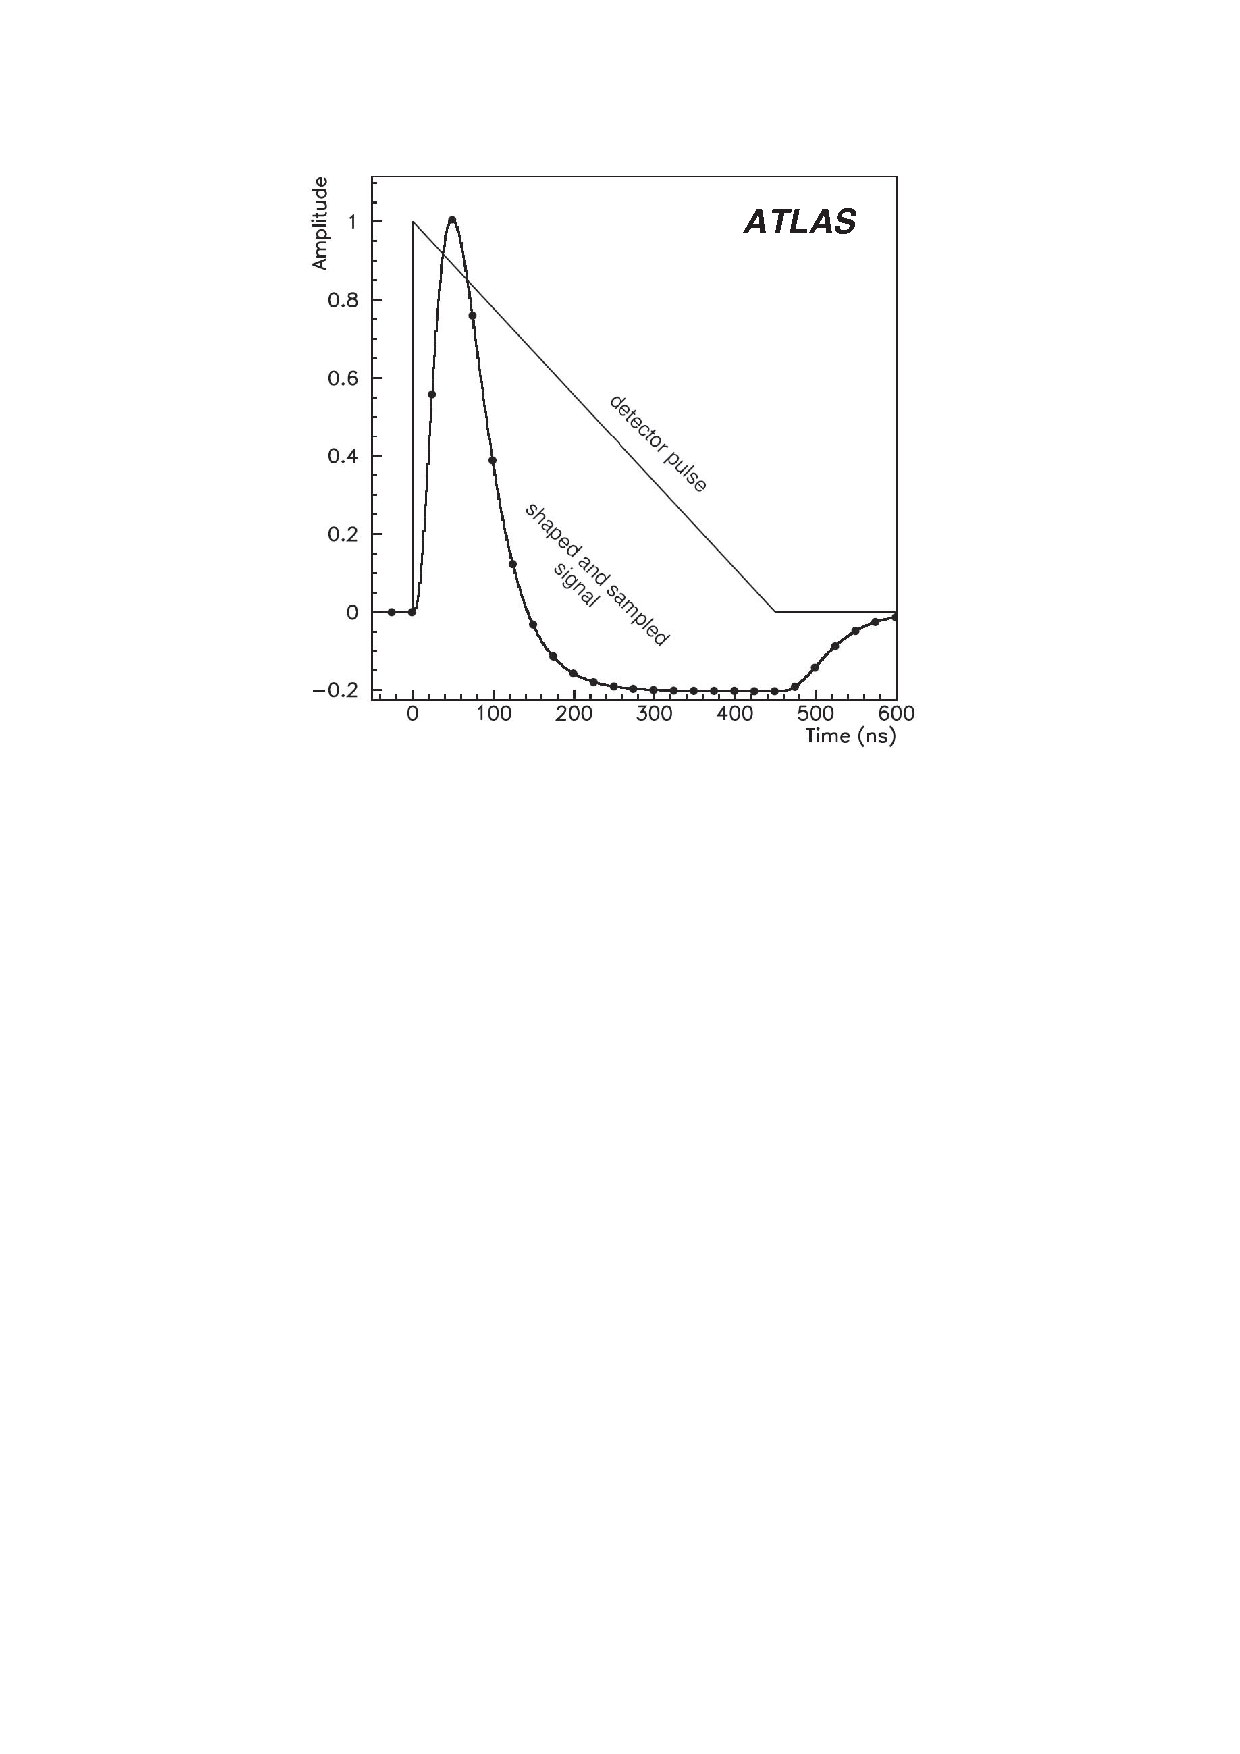
\includegraphics[width=0.5\textwidth]{figures/ATLAS/lar_pulse}
\caption[Liquid Argon calorimeter signal pulse]{The triangular pulse shape response from the LAr calorimeter, overlaid with the pulse after shaping and sampling.~\cite{ATLAS}.}
\label{fig:lar_pulse}
\end{center}
\end{wrapfigure}
%\end{figure}

In the region $|\eta|<2.5$, the EM calorimeters are segmented into three depth layers as shown in~\Fig{\ref{fig:lar_cross}}. The first ``strip'' layer provides precise $\eta$ measurements with a granularity of $\Delta\eta\times\Delta\phi=0.0031\times0.02545$. The fine $\eta$ segmentation helps differentiate photons from neutral pions decaying to two photons, and provides precise flight direction for neutral particles. The second layer has a coarser resolution of $\Delta\eta\times\Delta\phi=0.025\times0.0245$. However, it has a larger depth in order to absorb the bulk of the EM radiation in the showers. The final layer principally measures the remaining energy from the most energetic particles, while attempting to distinguish EM from hadronic objects. 

As the EM calorimeters sit outside the solenoid magnet, shower development has already begun by the time particles reach them. A separate, 11\,mm-thin pre-sampler layer of liquid argon sits in front of the solenoid magnet, and covers $|\eta|<1.8$. This permits earlier sampling of showers and provides a measurement of the energy lost in front of the calorimeter. 

The hadronic end-cap (HEC) also uses LAr as an active medium. However, it uses parallel copper plate absorbers instead of lead. Covering $1.5<|\eta|<3.2$, each HEC end-cap consists of two wheels with 32 identical wedge-shaped modules. The front (back) wheels have 24 (16) copper plates, each 25 (50)\,mm thick. The plates are kept with an 8.5\,mm gap between them, through which three electrodes create four drift zones. The front wheel has a granularity of $\Delta\eta\times\Delta\phi=0.1\times0.1$ while the back wheel has four times coarser granularity.

\begin{figure}[tb]
\begin{center}
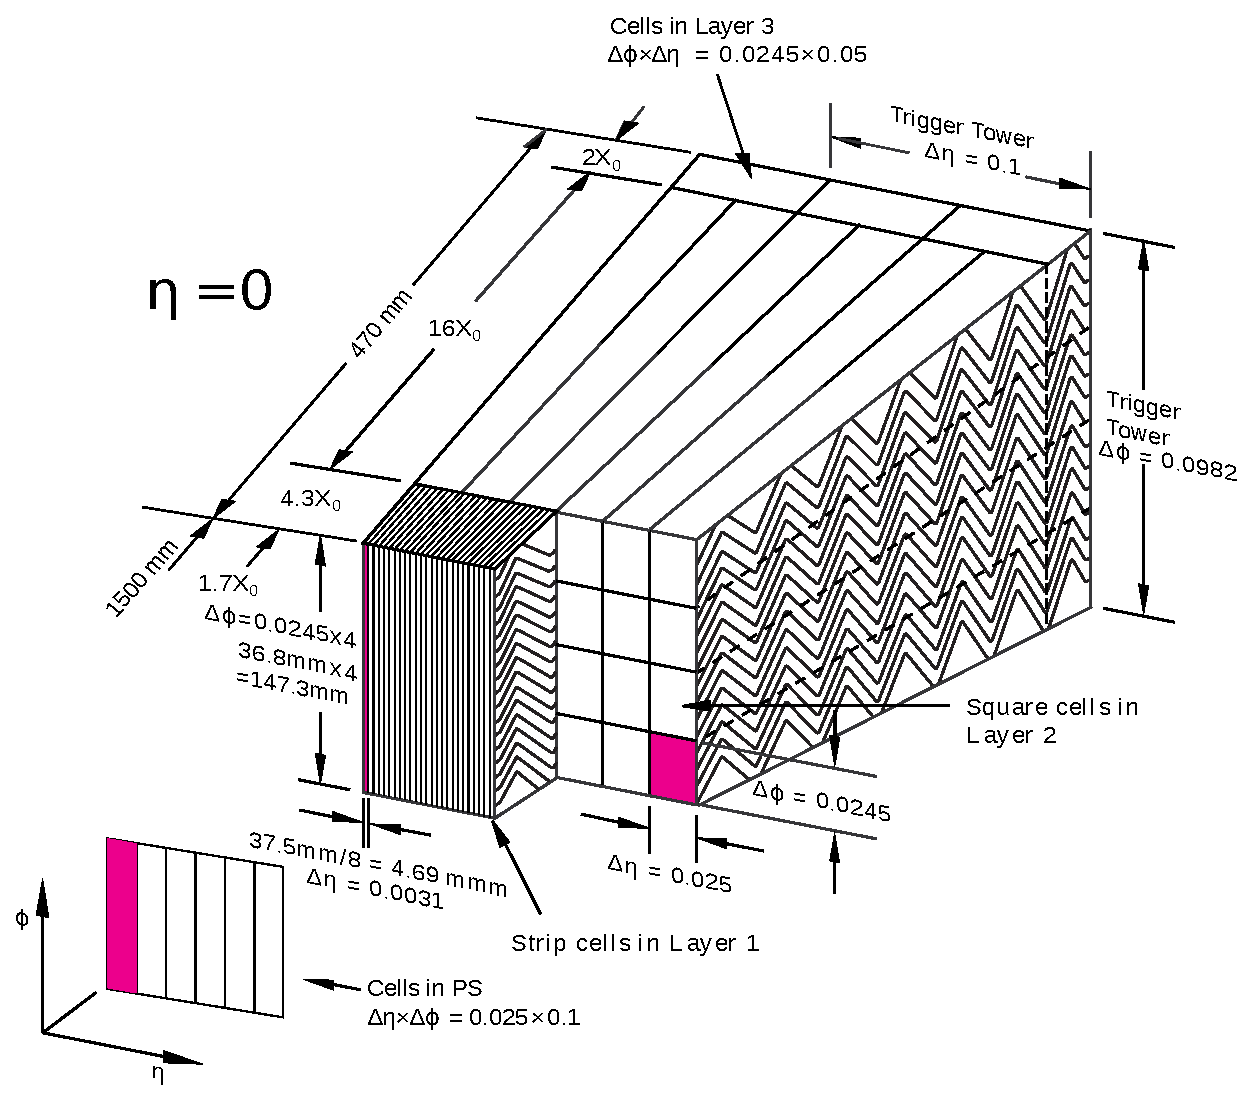
\includegraphics[width=0.8\textwidth]{figures/ATLAS/lar_cross}
\caption[Liquid Argon electromagnetic calorimeter layout]{Sketch of the accordion structure of the EM calorimeter showing the layers and granularity in $|\eta|$ and $\phi$~\cite{LAr_TDR}.}
\label{fig:lar_cross}
\end{center}
\end{figure}

%\begin{figure}[tbp]
%\begin{wrapfigure}{r}{0.52\textwidth}
%\begin{center}
%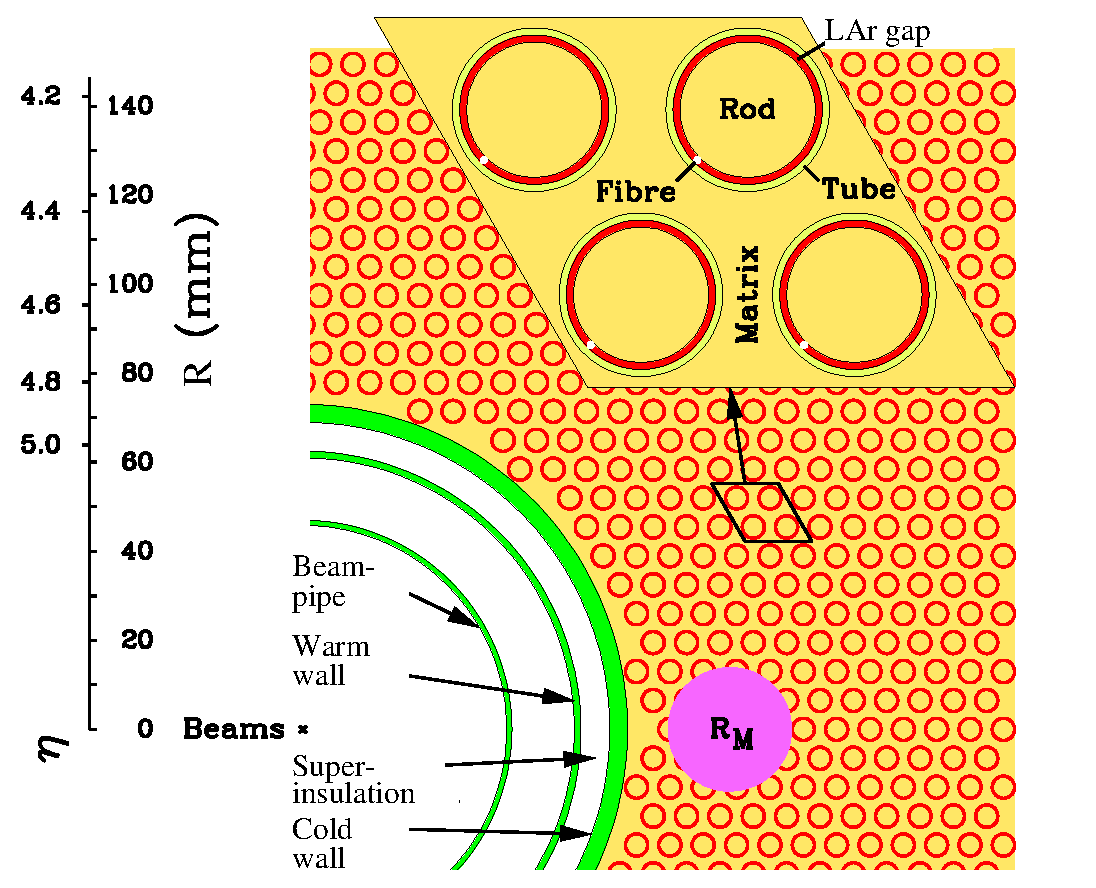
\includegraphics[width=0.5\textwidth]{figures/ATLAS/fcal_layout}
%\caption[LAr FCal structure]{FCal1 layout showing the LAr gap between the copper tubes and rods~\cite{ATLAS}.}
%\label{fig:fcal_layout}
%\end{center}
%\end{wrapfigure}
%\end{figure}

Sitting inside the HEC, the forward calorimeter (FCal) provides coverage from $3.1<|\eta|<4.9$. Due to its proximity to the beam pipe, the FCal experiences extremely large particle fluxes. To combat ion build-up, the LAr gap sizes are much smaller. Three 45\,cm deep modules make up the FCal: the first module (FCal1) is electromagnetic, while the two modules at larger $|z|$ (FCal2, FCal3) are hadronic. 
%Depicted in~\Fig{\ref{fig:fcal_layout}}, 
FCal1 consists of copper plates with holes drilled for cylindrical electrodes to pass through, parallel to the beam pipe. The electrodes consist of a copper rod inside a copper tube with a 269\,$\mu$m gap. Copper was chosen for FCal1 in order to quickly dissipate heat, while tungsten was chosen for the hadronic FCal2 and FCal3 modules in order to maximize containment of the hadronic showers. The FCal2 (FCal3) electrodes consist of a tungsten rod inside a copper tube with a 375 (500)\,$\mu$m gap and are surrounded by tungsten slugs. 

%
\subsection{Tile Calorimeter}
\begin{wrapfigure}{r}{0.52\textwidth}
\begin{center}
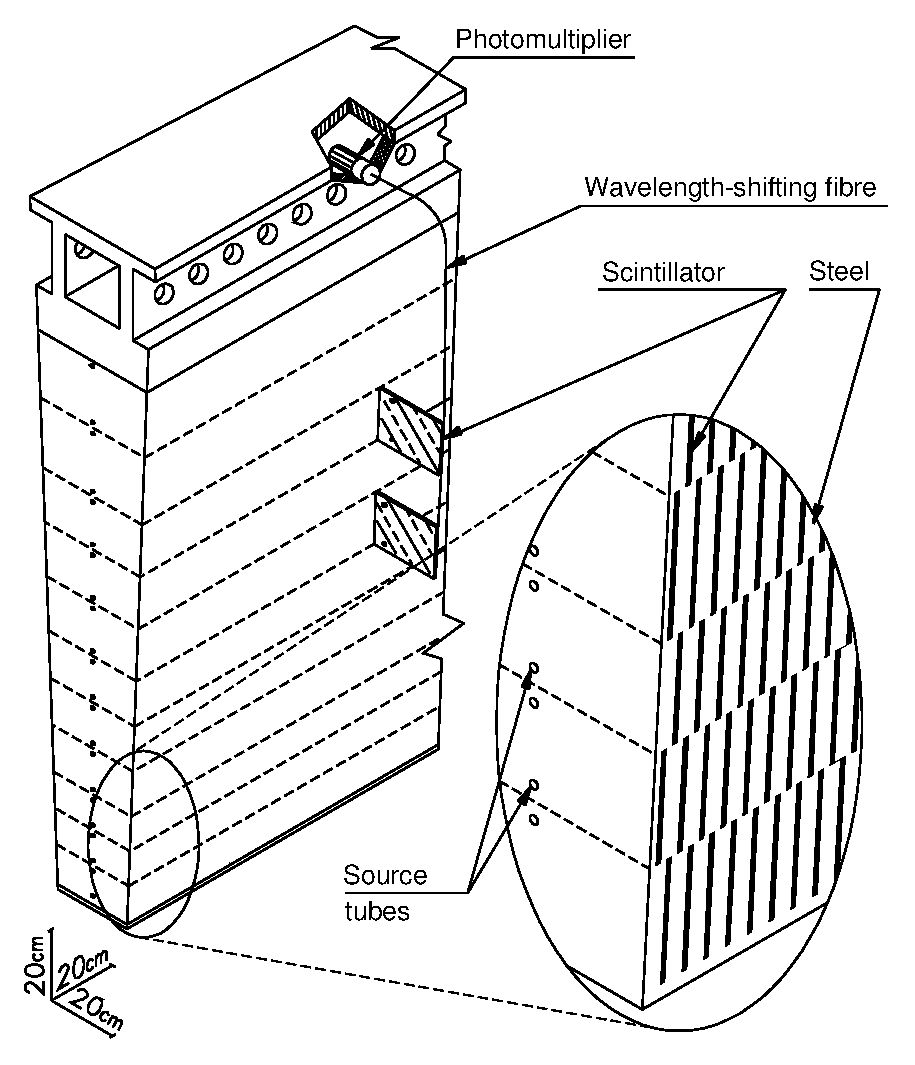
\includegraphics[width=0.5\textwidth]{figures/ATLAS/TileCal_Module}
\caption[Tile calorimeter module]{Layout of a wedge-shaped module in the Tile calorimeter with alternating steel absorber plates and plastic scintillating tiles~\cite{ATLAS}.}
\label{fig:tilecal}
\end{center}
\end{wrapfigure}
Sitting outside the LAr calorimeters in the barrel region is the hadronic Tile calorimeter, whose modules are shown in~\Fig{\ref{fig:tilecal}}. A 5.8\,m long main barrel covers $|\eta|<1.0$ and two 2.8\,m long extended barrels (EB) cover $0.8<|\eta|<1.7$. The cylindrical Tile calorimeter barrels extend radially from $R=2.28$\,m to $R=4.25$\,m, and are segmented into three depth layers. The hadronic Tile calorimeter is a sampling calorimeter consisting of steel absorber plates and scintillating plastic tiles serving as the active medium.

%\begin{figure}[htbp]

%\end{figure}

High energy particles striking the tile scintillators produce ultraviolet ``scintillation'' light, which is collected in wavelength-shifting fibres at either end of the tile. These fibres lengthen the wavelength of the ultraviolet scintillation to the visible spectrum and are fed into photomultiplier tubes. Groups of fibres are used to define read-out cells and three depth layers: cells in the two innermost depth layer have a granularity of $\Delta\eta\times\Delta\phi=0.1\times0.1$ while cells in the outermost layer have a granularity of $\Delta\eta\times\Delta\phi=0.2\times0.1$.

The main barrel and two EBs consist of 64 wedge-shaped modules that span $\Delta\phi=0.1$.  The plastic scintillator tiles are 3mm thick and vary in size depending on the radial position. In terms of interaction length, the thickness of the three depth layers of the main barrel (EB) are $1.5\lambda$, $4.1\lambda$, and $1.8\lambda$ ($1.5\lambda$, $2.6\lambda$, and $3.3\lambda$) from innermost to outermost. 

%%
\section{Muon Spectrometer}
As muons pass through the calorimeters, they lose much less energy than electrons to Bremsstrahlung radiation,
%\footnote{The total power radiated is inversely proportional to powers of the particle's mass.} 
and as a result, they are not contained in the calorimeters.
%\footnote{Also significant is that the muon lifetime is long enough to reach outside the calorimeters, as opposed to the heavy tau particles which decay in the ID.} 
Since muon tracks in the ID can suffer from poor momentum resolution at high \pt,
%\footnote{For very large \pt, tracks will have almost no curvature; thus, the accuracy of the momentum measurement will suffer.}
and relatively little muon energy is deposited in the calorimeters, a precision muon tracker~\cite{Muon_TDR} is placed outside the calorimeters to precisely measure muon momentum and position in the $R-z$ plane for $|\eta|<2.7$.  Additionally, muon triggering chambers are included to provide accurate bunch crossing identification and quick triggering decisions for $|\eta|<2.4$. The muon system is depicted in~\Fig{\ref{fig:mu_layout}}.  A summary of the coverage, resolution, and average number of hits for each component of the muon system is presented in~\Tab{\ref{tab:muon_cov}}.

\begin{figure}[htbp]
\begin{center}
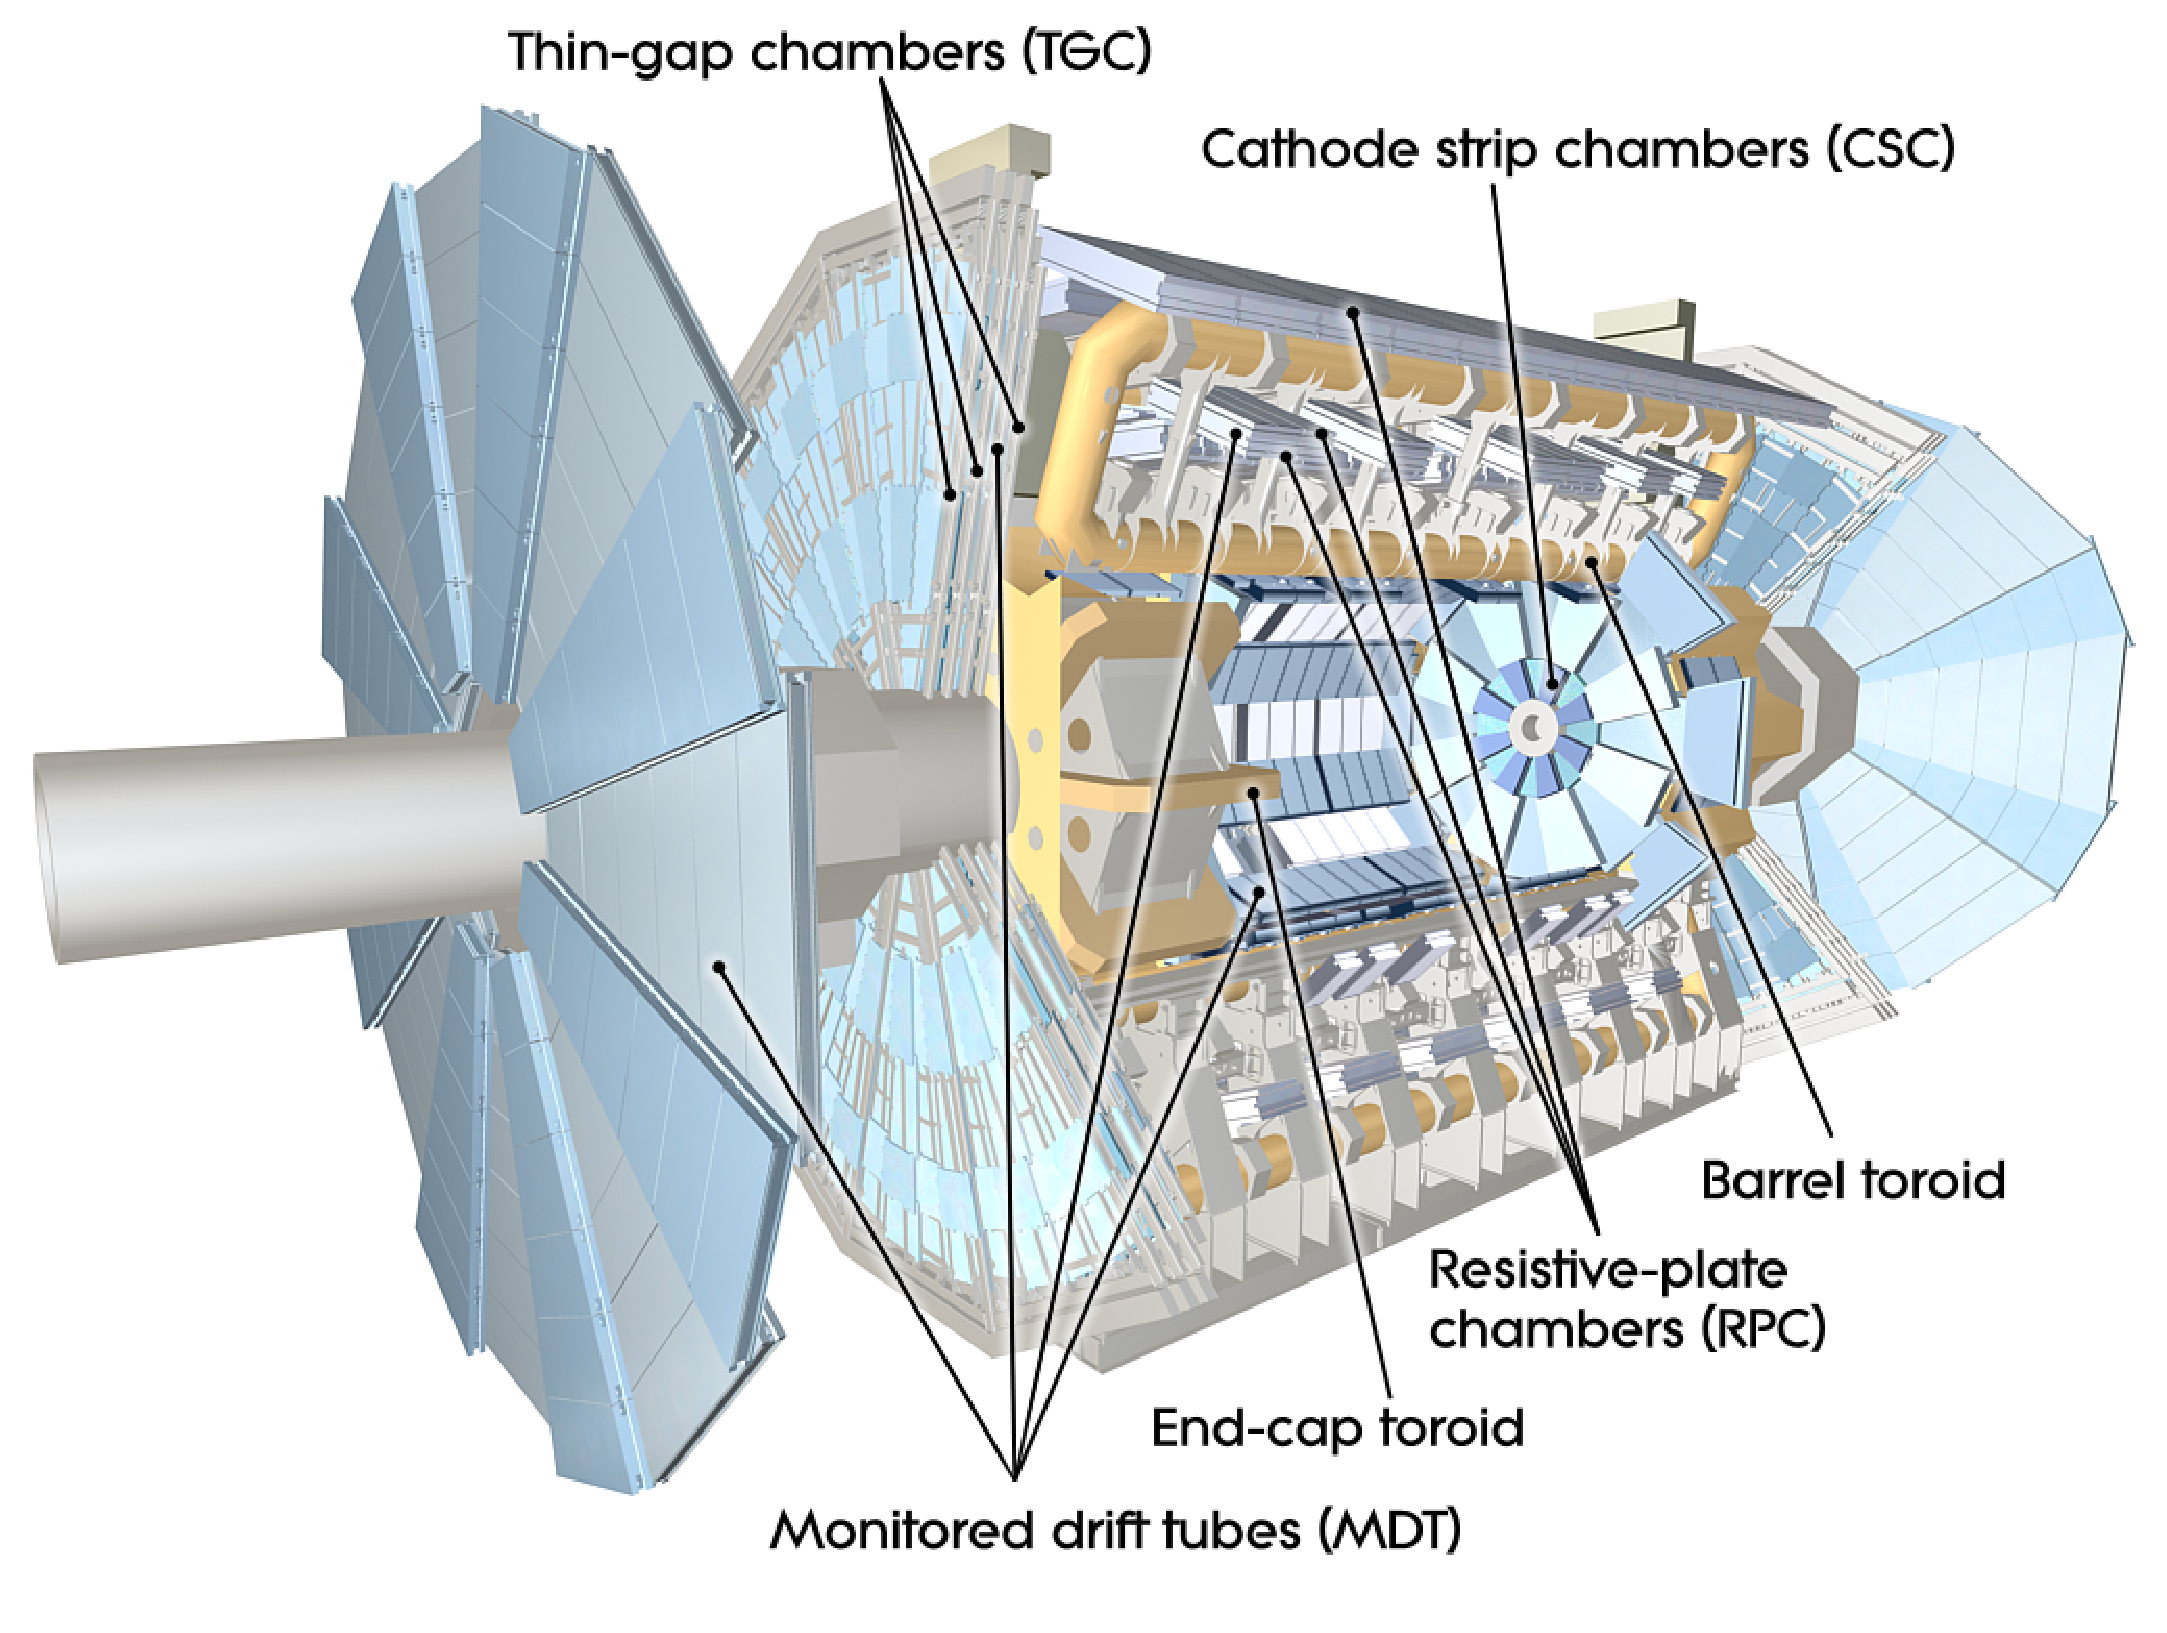
\includegraphics[width=0.8\textwidth]{figures/ATLAS/muon_layout}
\caption[Layout of Muon Spectrometer]{Diagram of the Muon Spectrometer~\cite{ATLAS}.}
\label{fig:mu_layout}
\end{center}
\end{figure}

\begin{table}[htbp]
\begin{center}
\begin{tabular}{lr|llll|ll}
\hline
%\vbox{\hbox{\strut \textbf{Component}}\hbox{\strut}}
\textbf{Sub-} &\textbf{Coverage} &\multicolumn{3}{r}{\textbf{Resolution}}&& \textbf{Avg.}&  \textbf{Type}\\
\textbf{detector}& & $z$ & $R$ & $\phi$ [mm] & $t$ [ns]& \textbf{Hits}&\\\hline\hline
MDT & $|\eta|<2.7$          & $35\,\mu$m & --- & --- &---& 20 & Precision \\
CSC & $2.0<|\eta|<2.7$   & --- & $40\,\mu$m & 5 & 7 & 4 & Precision \\
RPC & $|\eta|<1.1$        & $10$\,mm & --- & 10 & 1.5 & 6 & Trigger \\
TGC & $1.1<|\eta|<2.4$ & --- & 2-6 mm & 3-7 & 4 & 9 & Trigger \\
\hline
\end{tabular}
\caption[Coverage and performance of the muon system]{Summary of coverage, resolution, and function of each component of the Muon System.}
\label{tab:muon_cov}
\end{center}
\end{table}

%
\subsection{Precision Chambers}
In the barrel region, three layers of precision tracking Monitored Drift Tube (MDT) chambers in cylindrical shells are located on and between the eight toroidal barrel magnets, approximately at radii of $5$\,m, $7.5$\,m, and $10$\,m. In the end-cap region, wheels (with three layers) sit in front of and behind the end-cap toroidal magnets, approximately at $|z| =$ 7.4\,m, 10.8\,m, 14\,m, and 21.5\,m. The MDT is made out of pressurized 30\,mm diameter drift tubes filled with 93\,\% Ar and 7\,\% CO$_2$ gas at 3 bar. As passing muons ionize the gas, the electrons are collected on a centered, 50\,$\mu$m diameter tungsten-rhenium wire at a potential of 3080\,V. An MDT chamber consists of tubes grouped into three to eight layers where the tube (chamber) has a resolution in $z$ of 80 (35)\,$\mu$m. In order to try to avoid coverage gaps, 1,150 MDT chambers housing over 354,000 channels are arranged so that adjacent chambers overlap in $\phi$.

The Ar/CO$_2$ gas mixture has a relatively long drift time, reaching up to 700\,ns. This requires a large dead time
%\footnote{An interval in which the tube is no longer allowed to register a hit.} 
and leaves the tube susceptible to deteriorating resolution at high occupancies.
%\footnote{The slow drift time combined with high occupancies leads to ion build-up and a distortion of the electric field.}
The tubes will be expected to register hits up to 30\,kHz at nominal LHC operation due to backgrounds, including conversions of photons and neutrons.

To address the issues of high occupancy faced by the MDT in the forward region, Cathode Strip Chambers (CSC) are used on the innermost tracking layer for $2.0<|\eta|<2.7$. The CSC are multi-wire proportional chambers where the cathodes are segmented into strips, filled with an Ar (80\,\%) and CO$_2$ (20\,\%) mixture. The series of radial anode wires are separated by 2.5\,mm and sit between cathode sheets divided into 1.6\,mm strips. One layer of cathode strips is perpendicular to the anode wires, providing the precision coordinate with a resolution in $R$ of 60\,$\mu$m. The other layer is parallel to the anode wire, providing the transverse coordinate with a resolution in $\phi$ of 5\,mm. Charge collected on neighboring cathode strips is interpolated to derive a position measurement. In total, there are 32 CSC chambers with 31,000 channels.

The CSC chamber configuration allows for a much smaller drift time of 40\,ns, yielding a time resolution of 7\,ns.  While safe operation of the MDT can be reached with muon flux up to 150\,Hz/cm$^2$, the CSC can operate safely up to 1000\,Hz/cm$^2$. The chamber schematics of the MDT and CSC are shown in~\Fig{\ref{fig:muon_tracking}}.


\begin{figure}[htbp]
\begin{center}
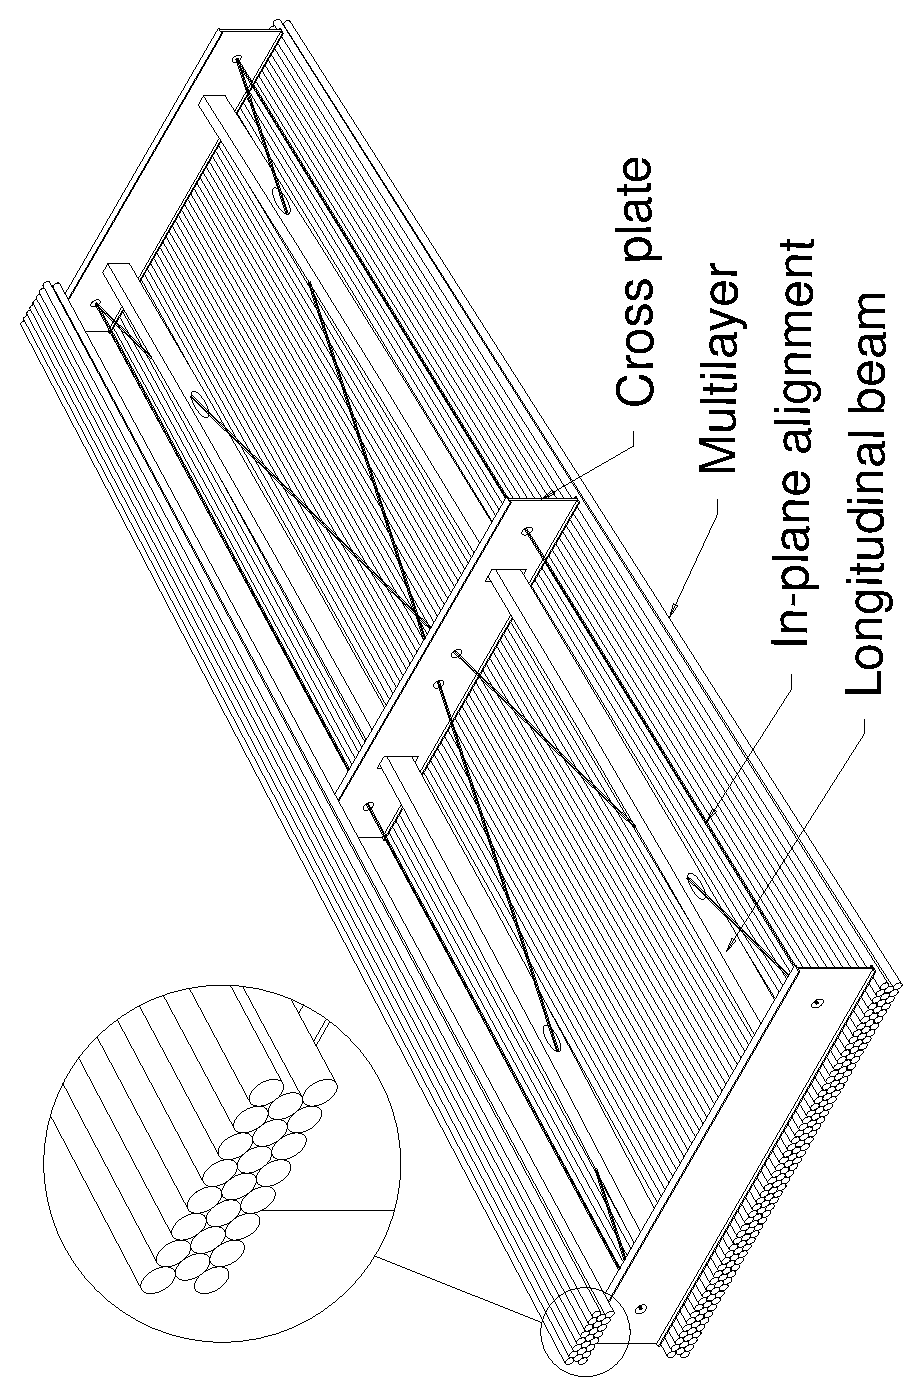
\includegraphics[angle=-90,origin=c,width=0.4\textwidth]{figures/Atlas/MDTchamber}
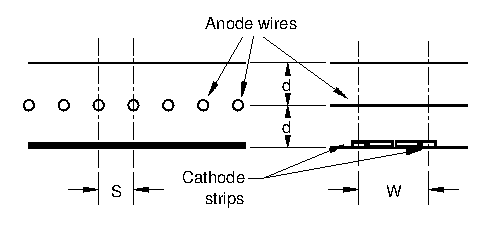
\includegraphics[width=0.59\textwidth]{figures/Atlas/CSC}
\end{center}
\caption[Schematic of muon precision tracking chambers]{A schematic of the MDT (left) and CSC (right) muon precision tracking chambers is shown~\cite{Muon_TDR}.}
\label{fig:muon_tracking}
\end{figure}

%
\subsection{Trigger Chambers}
In addition to the precision tracking capabilities provided by the MDT and CSC, the MS includes two triggering chambers, shown in~\Fig{\ref{fig:muon_trigger}}. 606 Resistive Plate Chambers (RPC) operate in the barrel region for $|\eta|<1.05$, while 3,588 Thin Gap Chambers (TGC) operate in the end-cap region for $1.05<|\eta|<2.4$. Due to the slow drift time of the MDT, assigning events to a specific bunch crossing requires additional input. The RPC and TGC were therefore designed to have sufficiently precise temporal resolution to assign muons to specific bunch crossings, making it possible to make event-by-event triggering decisions for specified \pt thresholds. Additionally, the coordinate of tracks perpendicular to the bending plane is provided by the triggering chambers.

The barrel RPC contain no wires: two resistive, parallel plates made of phenolic-melaminic plastic laminate are separated by 2\,mm with insulating spacers, while a gaseous mixture of 94.7\,\% C$_2$H$_2$F$_4$, 5\,\% Iso-C$_4$H$_{10}$, and 0.3\,\% SF$_6$ fills the interior. An electric field of 4.9\,kV/mm is applied between the plates, which facilitates avalanches
%\footnote{This is distinct from most other gas detectors in ATLAS which operate in proportional mode rather than avalanche mode.} 
from passing muons ionizing the gas. A thin layer of graphite is painted on the outside of the resistive plates, forming the HV and ground electrodes. Signals are read out via capacitively coupled pick up strips: 17\,$\mu$m thick copper strips are placed on the outside of the plates
%\footnote{The direction of the strips is perpendicular between the two plates.} 
with insulating 190\,$\mu$m PET film. Besides having a low operational voltage, the selected gas for the RPC has a low drift time, enabling a time resolution of 1.5\,ns. 

\begin{figure}[tb]
\begin{center}
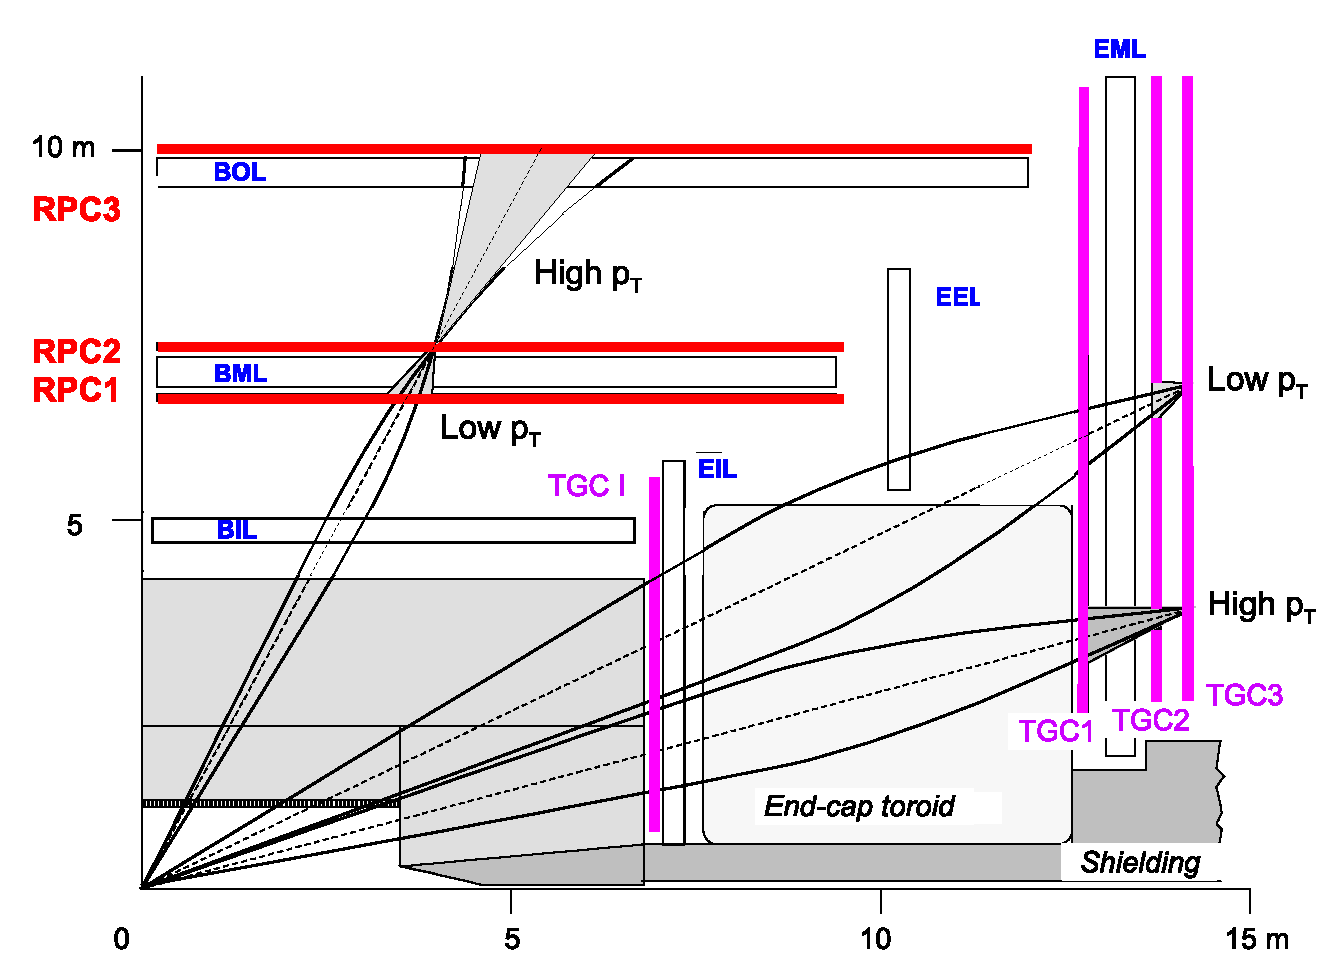
\includegraphics[width=0.8\textwidth]{figures/Atlas/RPC_TGC_schematics}
\end{center}
\caption[Schematic of muon trigger chambers]{Placement of the RPC and TGC layers is shown. RPC layers 1 and 2 book-end the middle MDT layer, and RPC layer 3 lies just outside the outermost MDT layer. TGC layers 1 and 2 surround MDT wheel 2 while TGC layer 3 is just beyond that. An additional TGC layer is placed just inside the end-cap toroid~\cite{ATLAS}.}
\label{fig:muon_trigger}
\end{figure}

In the forward region, the TGC faces several challenges: the end-cap sees ten times the radiation in the barrel, and no bending of muon tracks is provided as the chambers lie outside the end-cap toroidal magnet. To fulfill the triggering requirements, high granularity in $\eta$ and quick response time is achieved with the TGC, using identical principles to those in the multi-wire proportional chambers of the CSC. The gap is filled with a highly-quenching gaseous mixture of 55\,\% CO$_2$ and 45\,\% n-C$_5$H$_{12}$ (n-pentane), while the 50\,$\mu$m diameter gold plated tungsten anode wires are kept at a 2.9\,kV potential. In the TGC, the wire-to-cathode distance of 1.4\,mm is smaller than the wire-to-wire distance of 1.8\,mm, lending to a quick response. High spatial resolution is achieved by varying the number of wires grouped per read-out channel. 

\begin{figure}[tbp]
\begin{center}
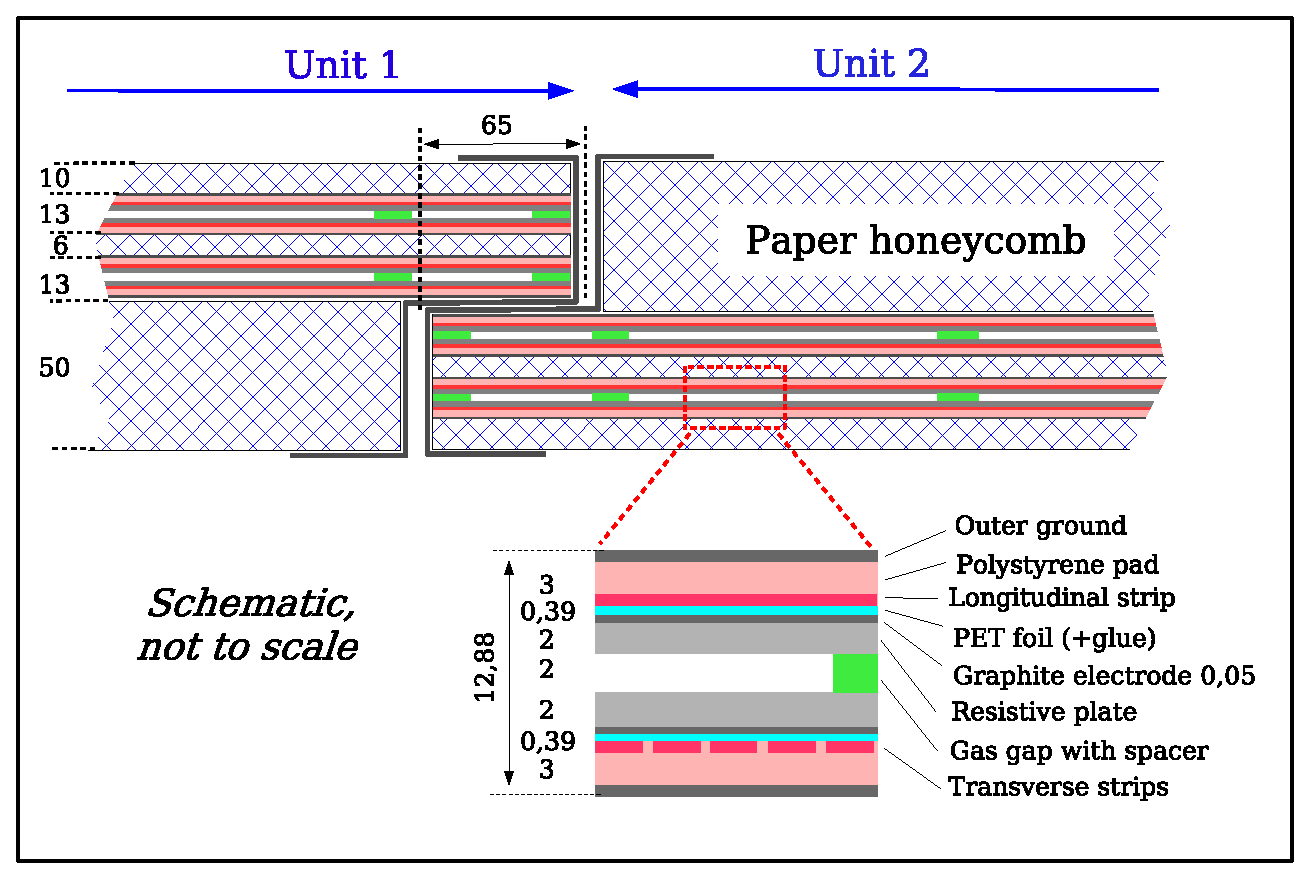
\includegraphics[width=0.4\textwidth]{figures/Atlas/RPC_structure}
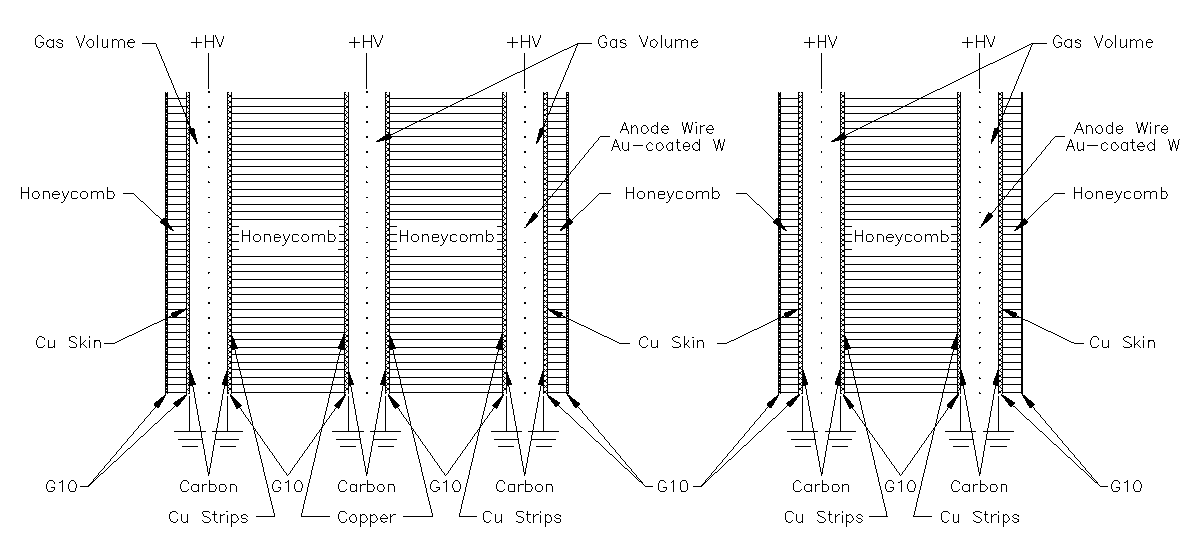
\includegraphics[width=0.59\textwidth]{figures/Atlas/TGC_structure}
\end{center}
\caption[Structure of the muon Resistive Plate Chambers and Thin Gap Chambers]{(left) Structure of the wireless resistive plate RPC and (right) multi-wire proportional chamber TGC~\cite{ATLAS}.}
\label{fig:muon_trigger_struct}
\end{figure}

The structure of the RPC and TGC modules are shown in~\Fig{\ref{fig:muon_trigger_struct}}. The triggering chamber $\phi$ measurement is used if the $\eta$ coordinate for a muon track in nearby MDT and triggering chambers match. There is a vanishing probability of more than one uncorrelated muon track per event in an MDT/triggering chamber pair.
%\footnote{If there are two uncorrelated tracks, it is ambiguous how to match the tracks.} 
However, two correlated, nearby muon tracks could appear from the decay of low mass particles, in which case the track must be matched with the ID. To control for fake rates, coincidence in both $\eta$ and $\phi$ is required for hits in all three triggering layers. In the RPC (TGC), layer 2 (layer 3) is used as a ``pivot-plane'' when determining triggering thresholds. A line from the IP to a hit in the pivot-plane is used as a reference for a straight-trajectory particle. Low (6-9\,\GeV) and high (9-35\,\GeV) \pt thresholds are determined by comparing the slope between hits in specified layers\footnote{
	The low (high) \pt threshold in the RPC is determined by measuring the slope between hits in layer 2 and layer 1 (layer 2 and layer 3). This slope is compared to the slope determined by the path from the IP to the hit in the pivot plane, layer 2. The trigger is passed if the difference in slope is above a threshold.
} and the slope of the reference straight-trajectory particle as depicted in~\Fig{\ref{fig:muon_trigger}}.


%%
\section{Forward Detectors}
Besides the detector systems already mentioned, three forward detectors are present, primarily to aid in luminosity measurements. The locations and coverage of the forward detectors are described in~\Tab{\ref{tab:fwd_loc}}. 

\begin{table}[tbp]
\begin{center}
\begin{tabular}{llr}
\hline
\textbf{Detector} & \textbf{Coverage} & \textbf{Dist. from IP} \\
&&($|z|$ [m]) \\\hline\hline
LUCID & $5.6 < |\eta| < 5.9$ &17\\
ZDC    & $8.3<|\eta|$ &140\\
ALFA  & $10.6 < |\eta|<13.5$ &240\\\hline
\end{tabular}
\end{center}
\caption[Location of forward detectors]{Location and coverage of the forward detectors.}
\label{tab:fwd_loc}
\end{table}

The Luminosity Measurement Using Cherenkov Integrating Detector (LUCID) measures inelastic $pp$ collisions in the forward region and primarily monitors the relative online luminosity.
%\footnote{A measure of the absolute luminosity is also possible with LUCID, but requires calibration either from simulation or other detector measurements.}. 
LUCID consists of 20 aluminum cones directed at the IP filled with C$_4$F$_{10}$ at 1.2-1.4\,bar, in order to measure Cherenkov radiation\footnote{
	Radiation emitted when charged particles travel through a dielectric medium faster than the phase velocity of light in that medium.
} from incident particles. By assuming the number of particles detected is proportional to the number of interactions in the bunch crossing, LUCID is able to measure $\mu$ in order to calculate the luminosity.  In Run II, the original LUCID detector was upgraded to LUCID-2~\cite{LUCID_2} to deal with several challenges: fast aging from a large total integrated luminosity, constraints on electronics from 25\,ns bunch crossings, increased particle fluxes saturating PMTs and counting algorithms, and a new beam pipe material\footnote{
	Moving from stainless steel to aluminum approximately increases the flux of particles through LUCID by a factor of four.
}. The new design no longer uses a gas, but rather quartz windows as the Cherenkov medium.


The Zero-Degree Calorimeter (ZDC) measures neutrons in the extremely forward region of $|\eta|>8.3$ for heavy-ion collisions.
%\footnote{ZDC can also help with low luminosity $pp$ collisions by measuring diffractive processes and aiding beam tuning.} 
ZDC plays an important role in determining the centrality
%\footnote{Centrality of heavy-ion collisions describes the amount of overlap between two colliding nuclei.} 
of heavy-ion collisions, since the number of neutrons in the forward region is highly correlated with the centrality of the collision. ZDC is a sampling calorimeter with tungsten absorber plates perpendicular to the beam line threaded with quartz rods, which serve as the active medium measuring Cherenkov radiation. 

The Absolute Luminosity For ATLAS (ALFA) detector determines the absolute cross section and luminosity by measuring elastic $pp$ scattering at an extremely small angle of 3\,$\mu$rad. The optical theorem relates the scattering amplitude in the extremely forward region to the exact cross section. The detector consists of scintillating fibres and sits inside a Roman pot
%\footnote{The name comes from the CERN Rome group at the Intersecting Storage Rings accelerator in the 1970's who first developed the technique.} 
which can be moved as close as 1\,mm from the beam axis. The detector can only be used during special runs with low emittance and high $\beta^{*}$.
%\footnote{Low emittance corresponds to particles confined tightly together with nearly the same momentum. High $\beta^{*}$ corresponds to a long tapering of the cross section of the beam, or low ``squeeze''.}

%%%
\iffalse
%%%
During the LHC shut down period between 2015 and 2016, part of the ATLAS Forward Proton (AFP) Detector~\cite{AFP_TDR} was installed, while the rest was installed between 2016 and 2017. The AFP is designed to measure forward protons from inelastic collisions, sitting  at $|z|=206$\,m (tracker) and $|z|=218$\,m (time-of-flight detector). The detectors are placed in Roman pots so they can be moved very close to the beam axis. The time-of-flight detector can help reduce pile-up by accurately determining the vertex position. The tracker sensors and read-out are based on the IBL 3D pixel sensors and FE-I4 chips.  At low luminosities, AFP is sensitive to diffractive events, while at high luminosities it is sensitive to anomalous couplings between photons and $W$ or $Z$ bosons. 
%%%
\fi
%%%

The Beam Conditions Monitor (BCM) helps with monitoring the beam stability and determining the luminosity.  If several proton bunches impact the collimators in front of the detectors, the large instantaneous radiation dose may cause severe damage. Thus, the BCM is designed to monitor the stability using precise time of flight measurements and trigger a beam dump if necessary. BCM modules consist of diamond sensors placed at $|z|=1.8$\,m and $R=5.5$\,cm. In Run-II, the Diamond Beam Monitor (DBM)~\cite{DBM} was added to complement the BCM, which can saturate at instantaneous luminosities of $10^{34}$\,cm$^{-2}$s$^{-1}$. The DBM, located approximately one meter from the IP, adds tracking capabilities with chemical vapor deposition diamond sensors. 


%%
\section{Magnet System}
The ATLAS magnet system~\cite{Magnet_TDR} allows for the measurement of the momentum of charged particles by bending their trajectories. The system consists of a central solenoid magnet, a barrel toroid magnet, and two end-cap toroid magnets, depicted in~\Fig{\ref{fig:mag_layout}}.

\begin{figure}[htbp]
\begin{center}
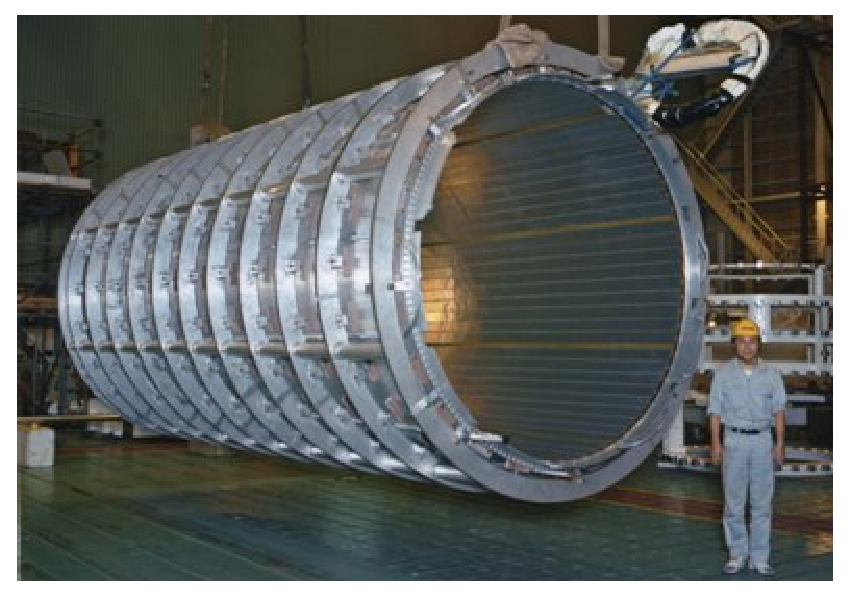
\includegraphics[width=0.48\textwidth]{figures/Atlas/sol_mag}
\includegraphics[width=0.51\textwidth]{figures/Atlas/bar_tor}
\caption[Photo of ATLAS solenoid and barrel toroid magnets]{The ATLAS solenoid magnet (left) after completion of the coil winding and barrel toroid magnets (right) after installation is shown, both next to a physicist for scale~\cite{ATLAS}.}
\label{fig:mag_layout}
\end{center}
\end{figure}

The central solenoid magnet surrounds the ID while sitting in front of the calorimeters. It provides a constant 2\,T axial field for the ID, and is relatively thin at 0.66\,$X_0$, to minimize energy losses and showering of particles before they enter the calorimeter. To minimize the material thickness yet still produce a strong field, the superconducting magnet uses Al-stabilized NbTi conductor wires wound inside an aluminum support. The 5 tonne solenoid magnet has over 9\,km of superconducting wire and measures 5.3\,m along the beam axis, with an inner diameter of 2.46\,m and an outer diameter of 2.56\,m.

%\begin{figure}[htbp]
\begin{wrapfigure}{r}{.51\textwidth}
\begin{center}
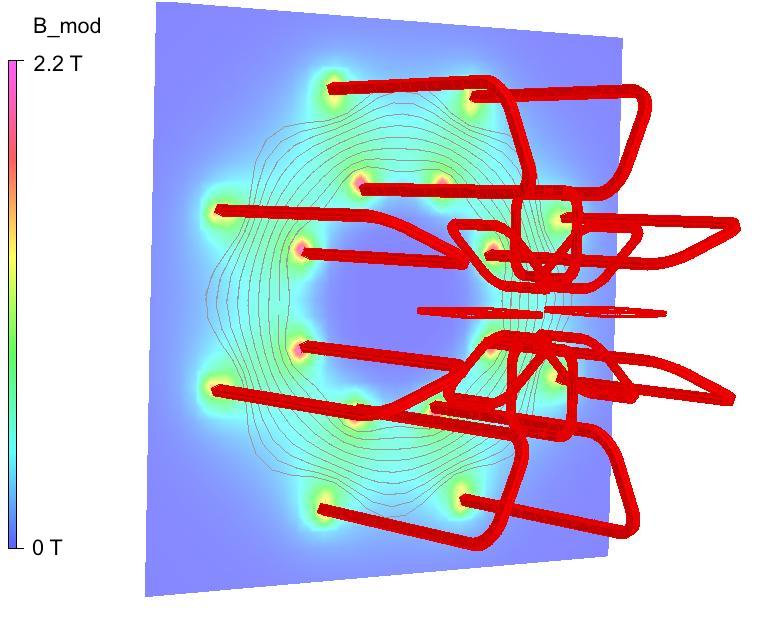
\includegraphics[width=0.5\textwidth]{figures/Atlas/atlas-ma-field}
\end{center}
\caption[Magnetic field of barrel toroid magnet]{The magnetic field of the barrel toroid magnet system at $z=0$~\cite{Atlas_mag}.}
\label{fig:atlas_magfield}
\end{wrapfigure}
%\end{figure}

The barrel toroidal magnet system consists of eight identical toroids azimuthally distributed around the beam axis. The system provides on average a 0.5\,T azimuthal field outside the calorimeters, shown in~\Fig{\ref{fig:atlas_magfield}}, to bend muons passing through the MS. The barrel toroid has over 100\,km of superconducting wire, with an envelope that is 25.3\, long with an inner diameter of 9.4\,m and an outer diameter of 20.1\,m.

Two end-cap toroid magnet systems sit on either side of the barrel toroid, to provide on average a 1.0\,T azimuthal field for muons in the end-cap region. The end-cap toroids can be retracted to access the inner subdetectors of ATLAS in the barrel region. The end-cap toroids are composed of eight flat square coils interspaced with keystone wedges. Each end cap toroid measures 5\,m along the beam axis, with an inner diameter of 1.7\,m and an outer diameter of 10.7\,m. 

%%
\section{Trigger and Data Acquisition}
Since data from one raw event is $\mathcal{O}$(1)\,MB\footnote{
	The event size increased from 1.6\,MB in Run-I to 2.4\,MB in Run-II in part due to a 20\,\% increase in read-out channels; however, the event size also depends on the pile-up. 
}, operating at the full LHC design frequency of 40\,MHz (25\,ns bunch spacing) corresponds to a total recording rate near $\mathcal{O}$(10)\,TB/s,
%\footnote{The exact rate fluctuates with the filling scheme, as not every bunch is filled with protons during normal operations.} 
if no filtering is implemented. Due to limitations in processing power and storage in the data acquisition system, however, this rate is intractable. The original design of the Trigger and Data Acquisition (TDAQ) system, utilized in Run-I, consists of a three level triggering system with a final recording rate of approximately 300\,MB/s. In Run-II, nearly all components received an upgrade, to maintain acceptably low \pt thresholds while dealing with increasingly challenging demands: increased center-of-mass energy from 8\,\TeV\,to 13\,\TeV, increased pile-up ($\mu$), decreased bunch spacing interval from 50\,ns to 25\,ns, and increased instantaneous luminosity~\cite{trigger_2015, trigger_evo}. The Run-II TDAQ architecture and parameters are shown in~\Fig{\ref{fig:tdaq_run1_run2_v2}} and~\Tab{\ref{tab:tdaq_run1_run2}}.

\begin{wrapfigure}{r}{.51\textwidth}
\begin{center}
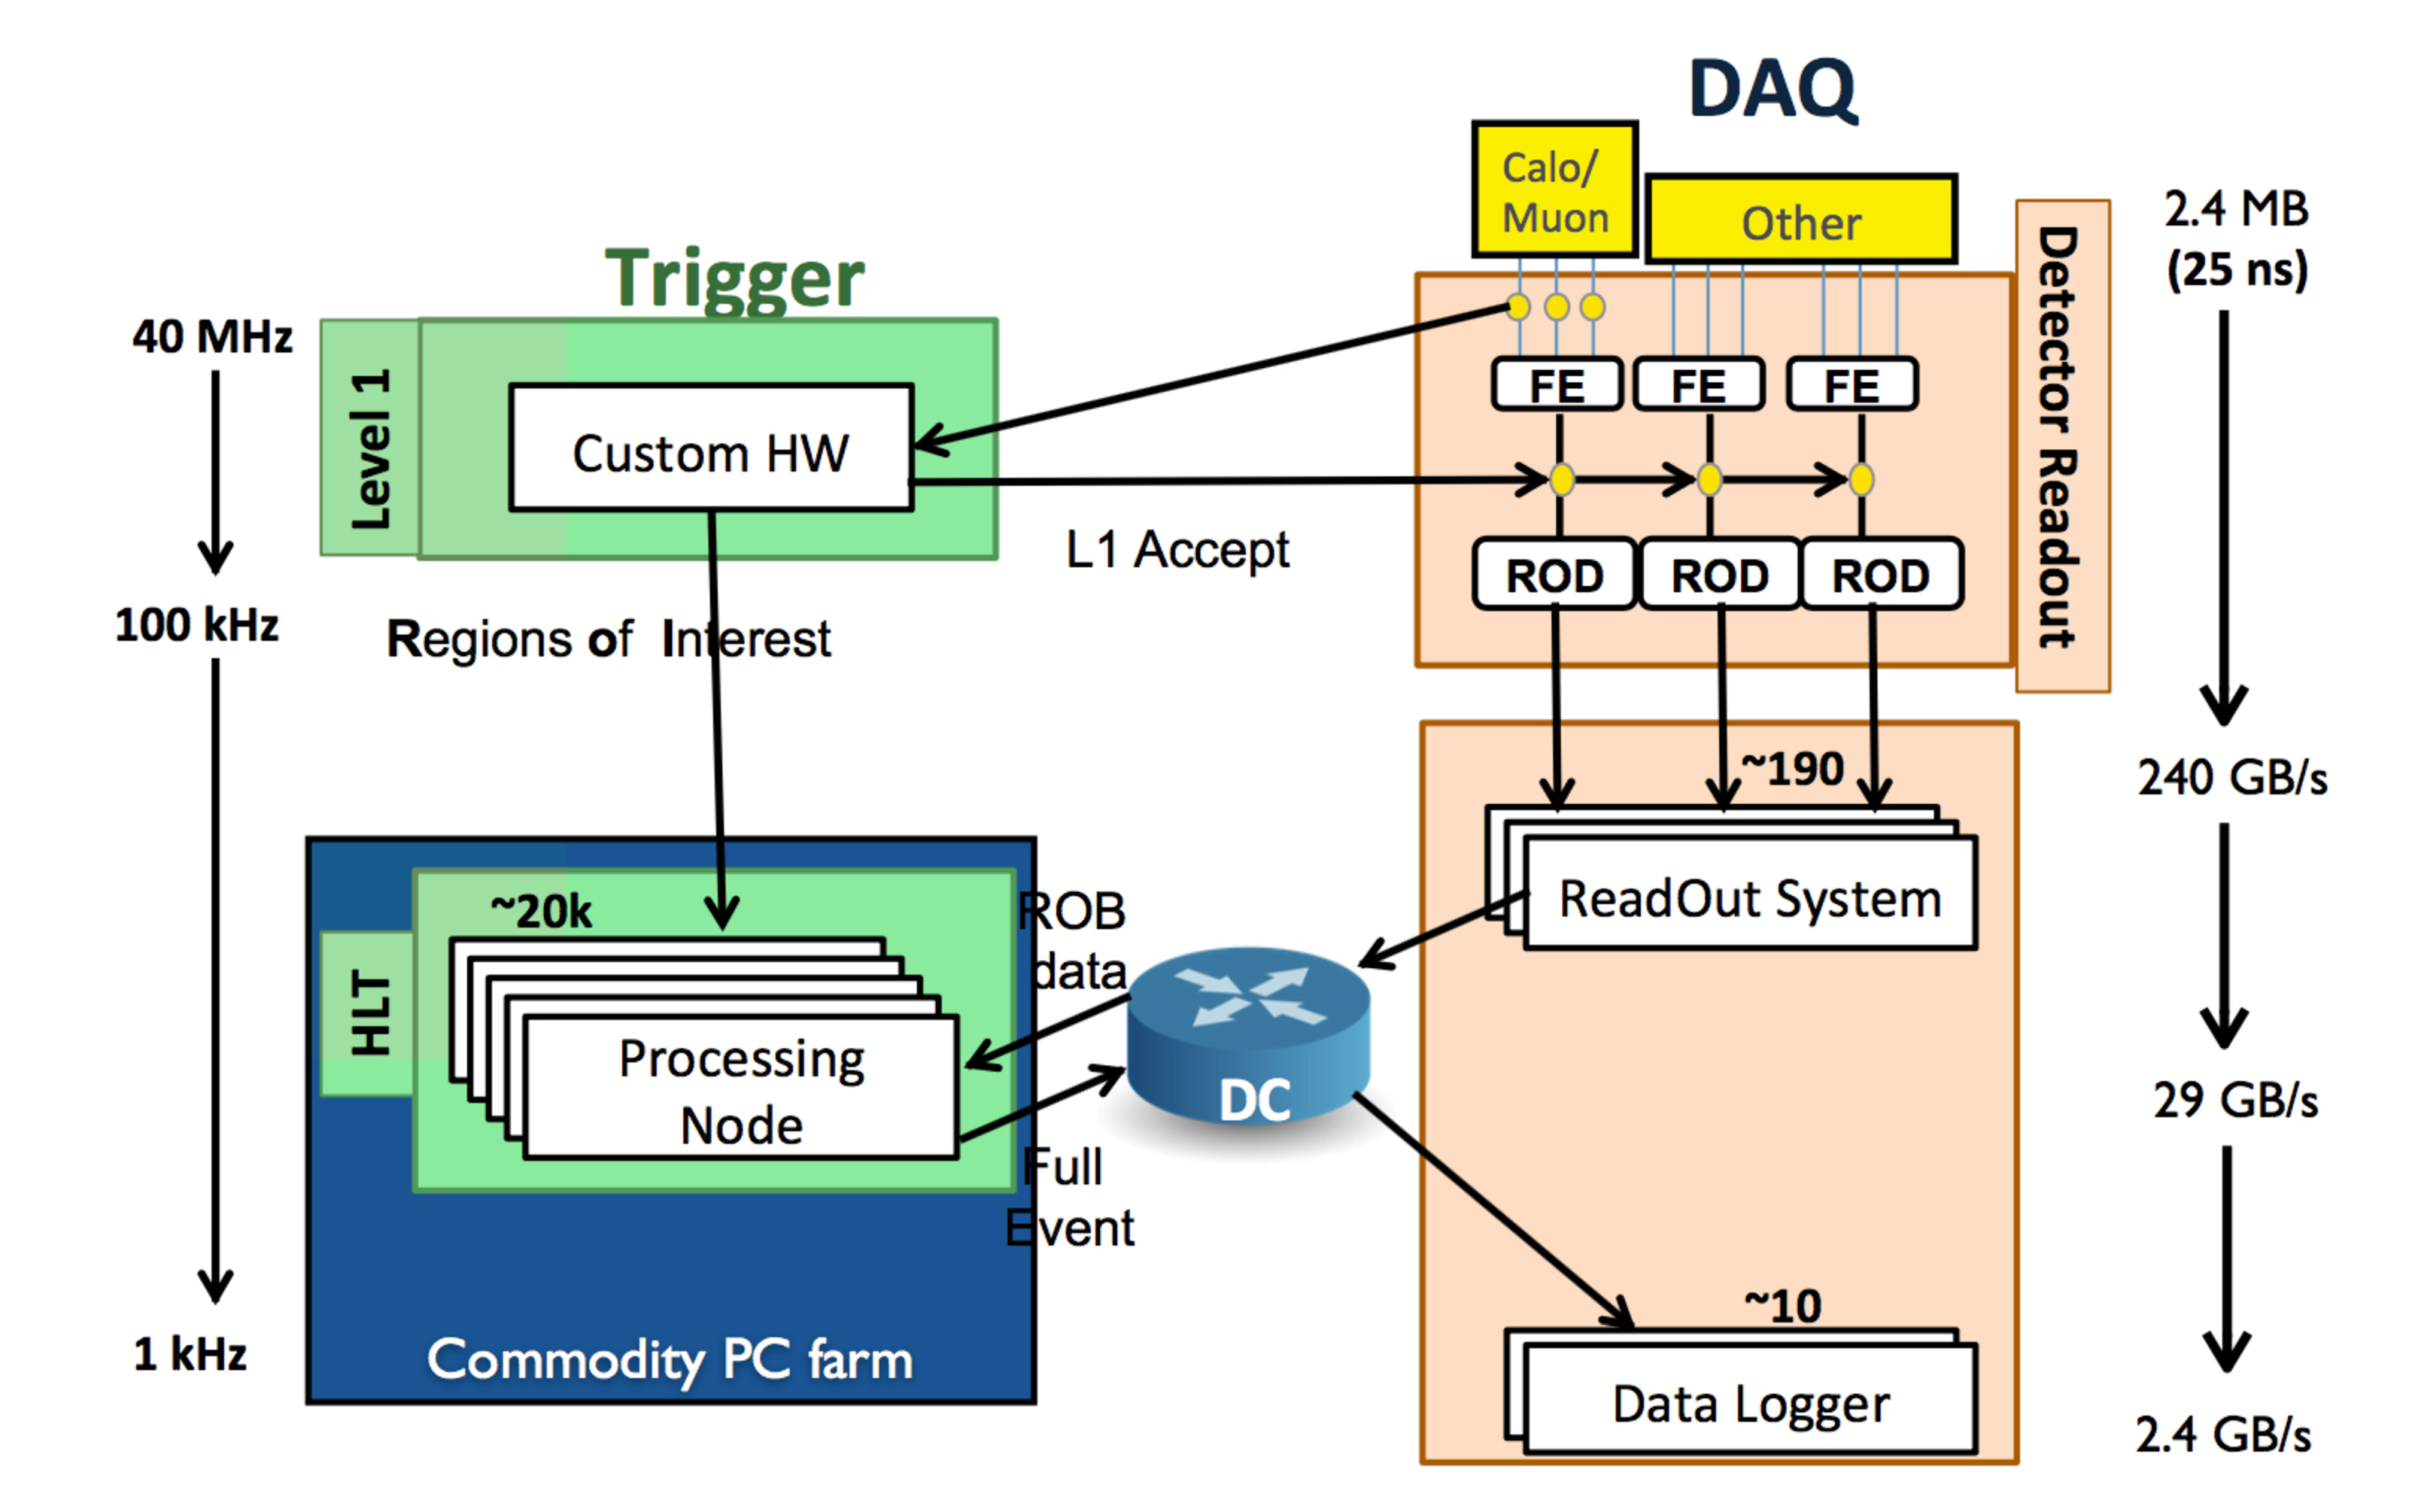
\includegraphics[width=0.49\textwidth]{figures/Atlas/tdaq_run2_v1}
\end{center}
\caption[Trigger and Data Acquisition architecture in Run-II]{The TDAQ architecture was modified in Run-II by consolidating the Level-2 and Event Filter stages into one High Level Trigger stage. The total event rate increased from 600\,Hz in Run-I to 1\,kHz in Run-II, in a more challenging environment, with the help of the upgrades and optimizations implemented~\cite{trigger_evo}.}
\label{fig:tdaq_run1_run2_v2}
\end{wrapfigure}

The first level of the trigger system is a hardware-based Level-1 (L1) trigger which slims the 40\,MHz input event rate to a 100\,kHz output rate.
%\footnote{Although the L1 rate has increased from Run-I, the 100\,kHz output rate is hardware-limited by the read-out capabilities of the ATLAS subdetectors; thus, in future upgrades of the LHC, the trigger architecture and detector read-outs will need upgrades to accommodate the ever-increasing luminosity and $\mu$.} 
The L1 trigger tries to identify high-\pt electrons, photons, muons, jets, and hadronically decaying $\tau$-leptons, as well as large \MET and $E_{\rm T}^{\text{tot}}$. Sums of calorimeter energy deposits from 7000 trigger towers, with an approximate granularity of $\Delta\eta\times\Delta\phi=0.1\times0.1$, are collected by the ``L1Calo'' trigger, while RPC and TGC track information is collected by the ``L1Muon'' trigger.  A ``trigger menu'' consisting of 512 ``trigger items'', logical combinations of trigger inputs from L1Calo and L1Muon, is processed by the Central Trigger Processor (CTP) which produces a trigger decision within 2.5\,$\mu$s. Event data must be buffered while the L1 trigger decision is being formed. The trigger items in the trigger menu can be ``pre-scaled'' so that a predetermined fraction of events passing the trigger item are randomly ignored, thereby reducing the overall trigger rate. The CTP is also responsible for limiting the time between L1 accepts (simple dead time) and a leaky bucket algorithm to limit the number of L1 accepts in a given number of bunch crossings (complex dead time)~\cite{Leaky_bucket}. A detector may issue a ``busy'' signal to the CTP in order to signal that its buffers are full, preventing further L1 accepts until the busy signal is cleared.
\begin{table}[tbp]
\begin{center}
\begin{tabular}{lrr}
\hline
Property & Run-I & Run-II \\\hline\hline
$\sqrt{s}$ [\TeV] & 8 & 13\\
L$_{\text{peak}}$ [$10^{33}$\,cm$^{-2}$s$^{-1}$] & $5.0$ & $13.8$\\
Bunch spacing [ns] & 50 & 25 \\
\# bunches & 1380 & 1380-2700\\
Avg. pile-up & 20.7 & 24.9 \\
Event size [MB] & 1.6 & 2.4 \\
L1 inputs (items) & 160 (256) & 512 (512) \\
L1 rate [kHz] & 70 & 100 \\
Total output rate [kHz (GB/s)] & 0.6 (0.96) & 1.0 (2.4) \\
\hline
\end{tabular}
\end{center}
\caption[Trigger and Data Acquisition parameters in Run-I and Run-II]{Comparison of LHC and TDAQ parameters between Run-I and Run-II (up to 2016). The increased luminosity, center of mass energy, and pile-up required updated algorithms and architecture to address the increased production rate and keep the output rate reasonable.}
\label{tab:tdaq_run1_run2}
\end{table}

Event data is buffered on detector-specific front-end electronics until a L1 trigger decision is received. Upon an L1 accept, the next stage in the data acquisition system is the transfer of the buffered event data to a read out system (ROS) at approximately 240\,GB/s. A data collection (DC) system interfaces with fragments from the ROS to provide requested event information to the next level of the trigger, the High Level Trigger (HLT). 

The second level of the triggering system is the software-based HLT\footnote{The current HLT performs the combined functions of the Run-I Level-2 trigger and Event Filter.}, which reduces the 100\,kHz L1 rate to a final 1\,kHz event output rate, with an average latency of 200\,ms. The HLT uses regions of interest (ROI) identified by the L1 trigger (approximately 2\,\% of the total event data) to access full or partial event information from the ROS through the DC interface. The L1 ROIs seed a system of approximately 2500 ``trigger chains'' in the HLT: a sequence of algorithms which increase in complexity and require more detector information. The HLT has access to full granularity calorimeter information, precision muon measurements, and ID tracking information, all of which is unavailable to the L1 trigger. The HLT utilizes a two-pass approach: a first quick reconstruction rejects the majority of events, and a second slower, more precise reconstruction filters the remaining events. Pending an HLT accept, event data buffered in the ROS is transferred to the Tier-0 storage facilities at CERN at 2.4\,GB/s for full offline event reconstruction. 

